\documentclass[../tesis_main.tex]{subfiles}


\chapter{Resultados y conclusiones}

La descripción de las pruebas y la discusión de resultados se abordará con la siguiente estructura. Se describirán pruebas que permitieron realizar una evaluación del desepeño de los algoritmos con respecto a los que actualmente están operando en el robot de servicio Justina.\\

Se describirá conforme al desarrollo de este estrabajo. 

\begin{enumerate}
	\item{Extracción de planos.}
	\begin{itemize}
		\item{Exactitud, rapidez.}
	\end{itemize}

	\item{Extracción de objetos y sus características.}
	\begin{itemize}
		\item{Exactitud en la estimación de la posición.}
		\item{Comparación en caracteristica de altura.}
		\item{Estimación de la orientación de objetos.}
		\item{Exactitud en el cálculo de la orientación. Comparación orientación estimada y real.}
	\end{itemize}


	\item{Espacio de trabajo del algoritmo númerico.}
	\item{Comparación tarea de manipulación utilizando información de orientación de los objetos.}
\end{enumerate}



\newpage
%%%%%%%%%%%%%%%%%%%%%%%%%%%%%%%%%%%%%%%%%%%%%%%%%%%%%%%%%%%%%%%%%%%%
%%%%%%%%%		EXTRACCIÓN DE PLANOS           %%%%%%%%%%%%%%%%%%%%%
	\section{Extracción de planos.}

	En esta sección analizaremos los resultados obtenidos al probar el algoritmo RANSAC para encontrar planos modificando el numero de iteraciones. Observaremos el comportamiento del error y el tiempo de ejecución a fin de encontrar el número óptimo de iteraciones para este algoritmo.\\

	El proceso para el análisis de datos fue el siguiente: se propuso un modelo de plano conocido por el usuario. Dicho modelo se obtuvo a partir del conocimiento de la altura del plano en este caso una mesa. Posteriormente se cuantificó la cantidad de puntos que entraban en este modelo ideal y se tomó como base para la medición de errores. Continuando con el procedimiento se modificó el algoritmo para realizar un número determinado de iteraciones (600, 200, 100, 50, 30, 24 y 20) y se midió el error relativo y el tiempo de ejecución, en cada uno de estos procedimientos.\\

	Para probar el algoritmo con 600 iteraciones se tomaron 50 muestras los resultados se pueden observar en la siguiente gráfica.\\


	\begin{figure}[H]
		\begin{minipage}{18cm}
		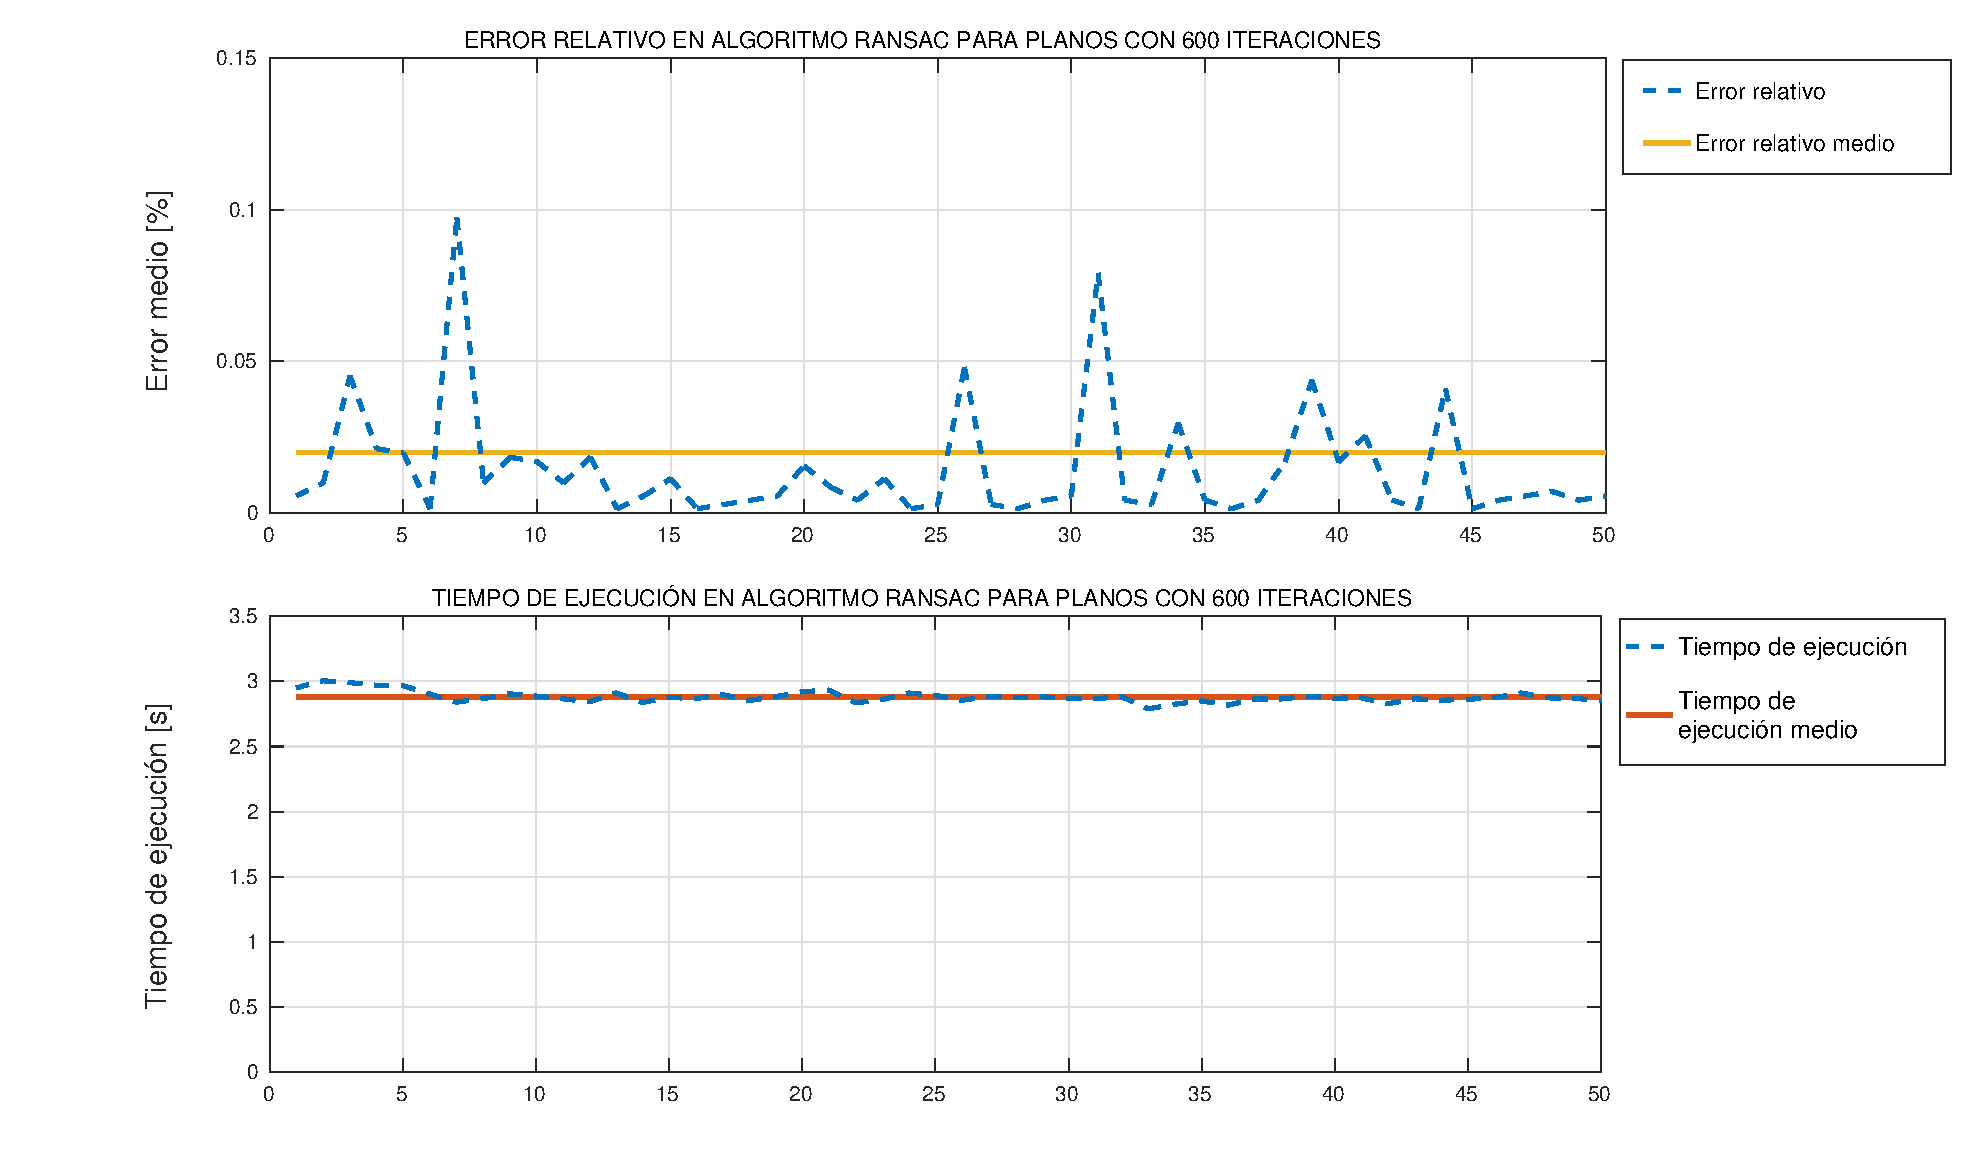
\includegraphics[width=16.0cm, height=9.0cm]{resultados/ransac_600}	
		\end{minipage}
		\begin{center}
		\caption{Gráfica correspondiente al error relativo para el algoritmo RANSAC para detección de planos con 600 iteraciones.}
		\end{center}
	\end{figure}
	
	\begin{figure}[H]
		\begin{minipage}{18cm}	
		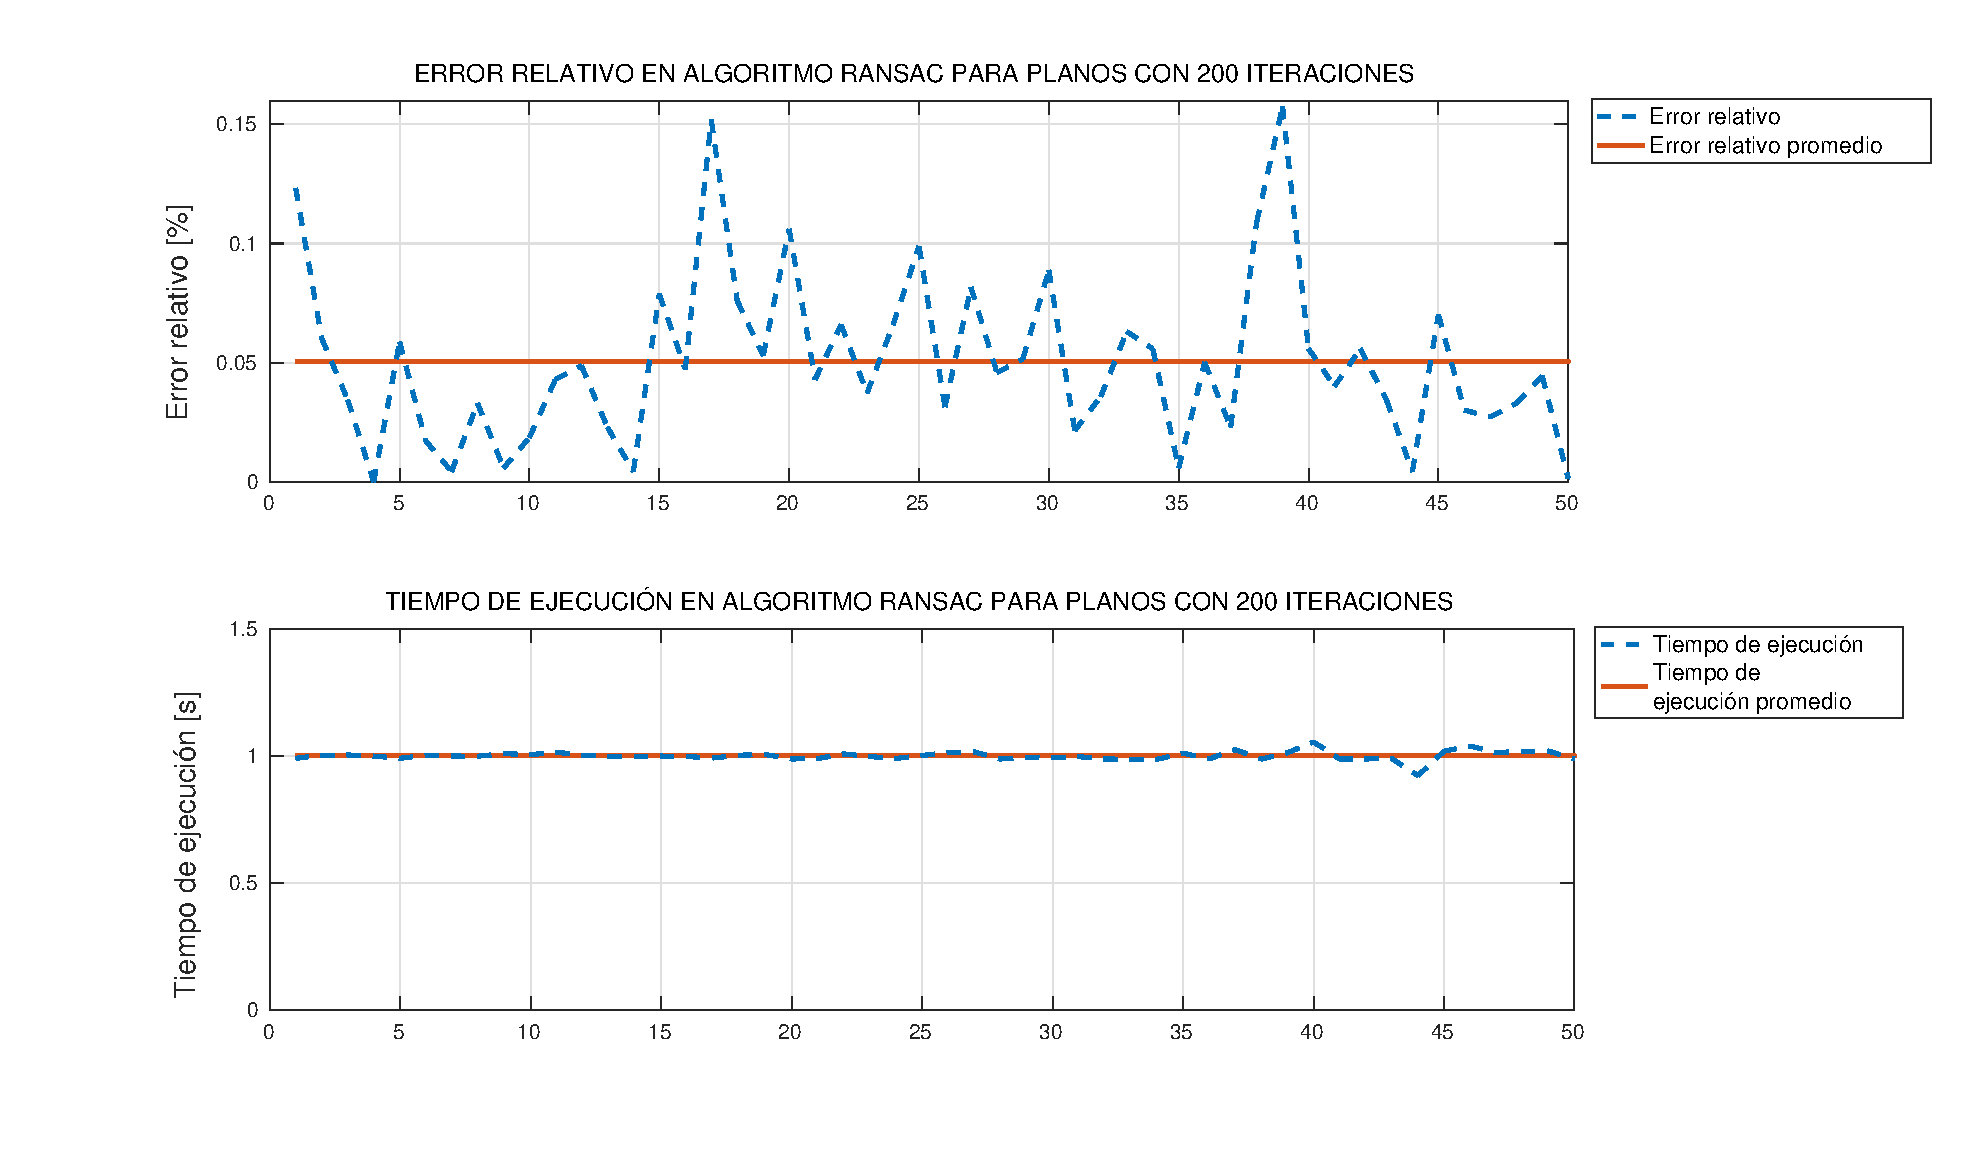
\includegraphics[width=16.0cm, height=9.0cm]{resultados/ransac_200}	
		\end{minipage}
		\begin{center}
		\caption{Gráficas correspondientes al error relativo y tiempo de ejecución para el algoritmo RANSAC con 200 iteraciones.}
		\end{center}
	\end{figure}

	\begin{figure}[H]
		\begin{minipage}{18cm}
		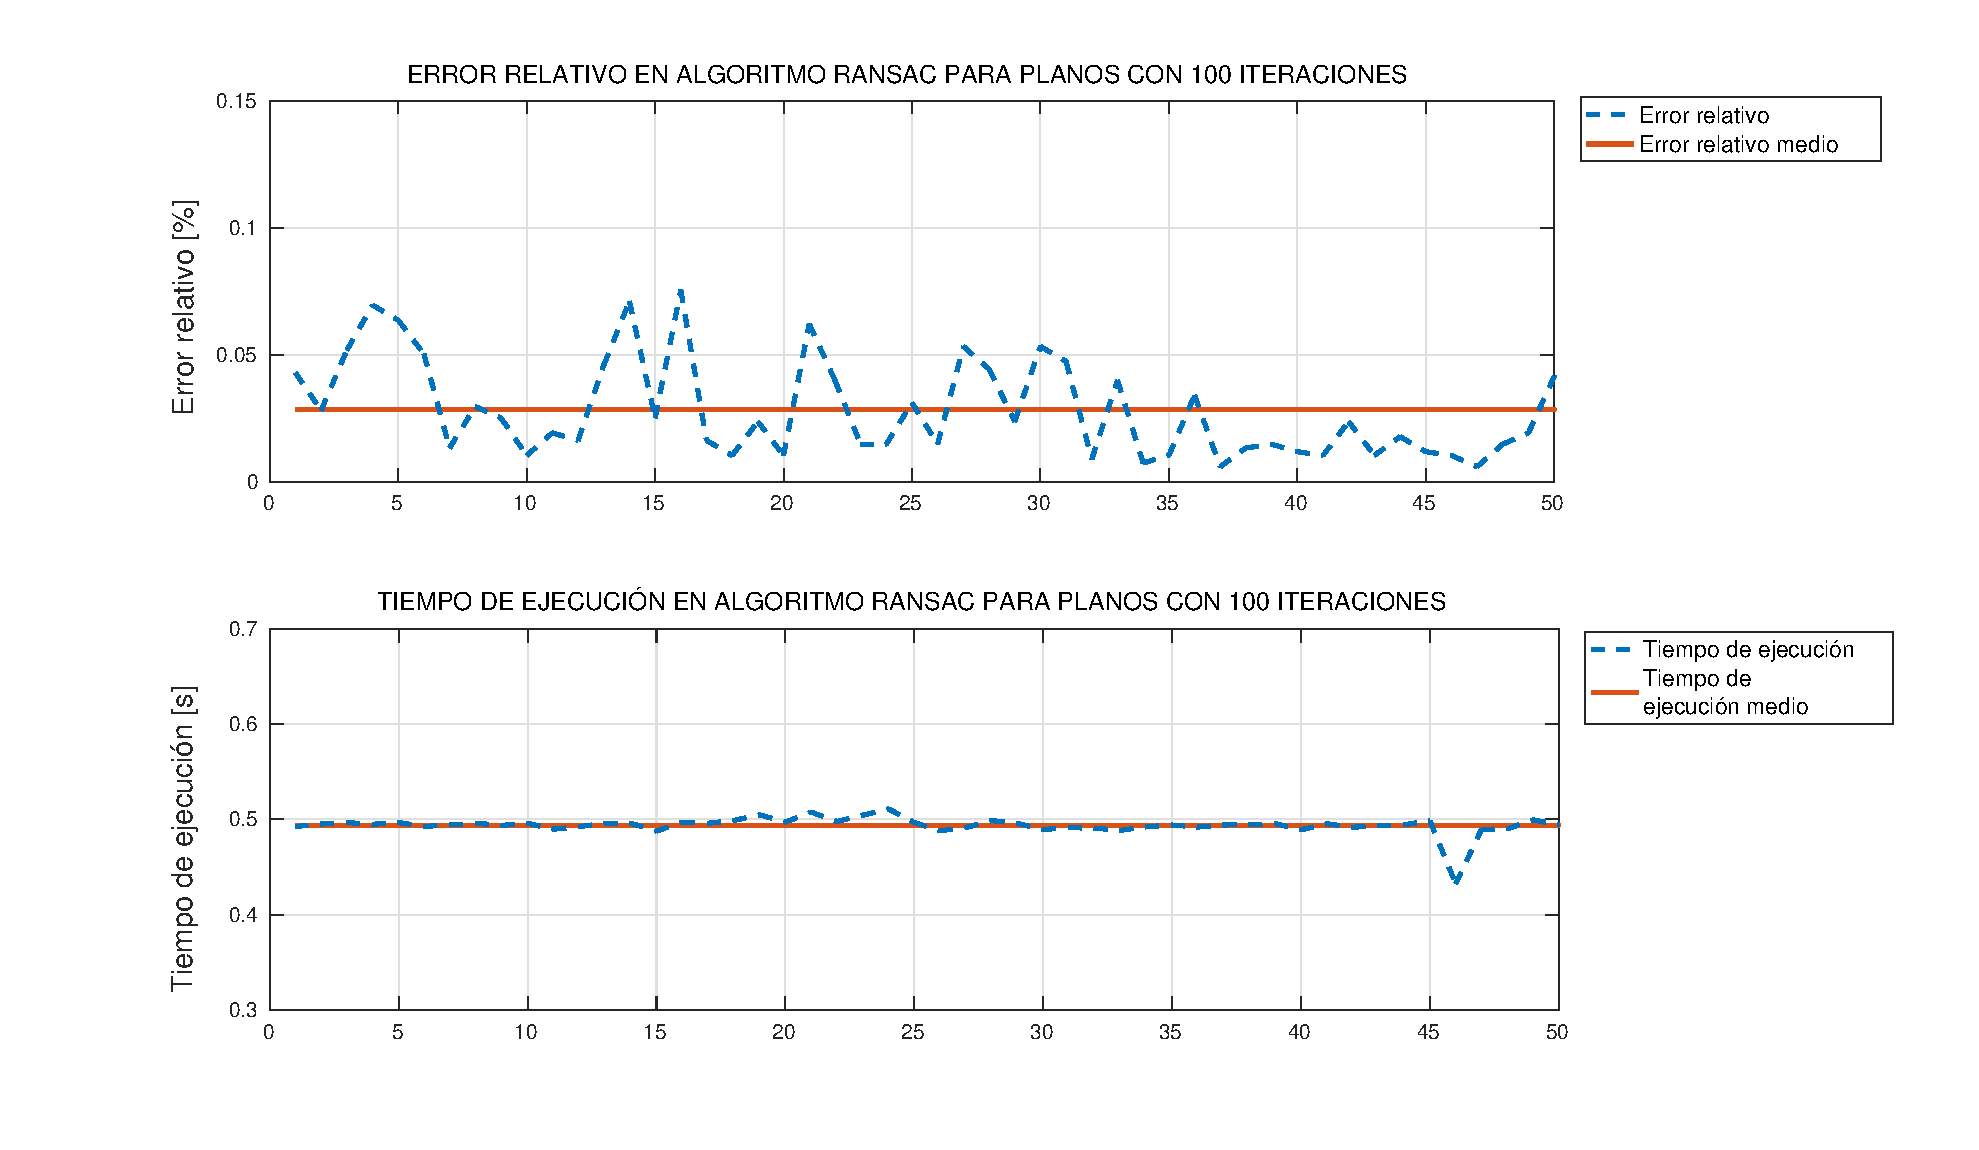
\includegraphics[width=16.0cm, height=9.0cm]{resultados/ransac_100}
		\end{minipage}
		\begin{center}
		\caption{Gráficas correspondientes al error relativo y tiempo de ejecución para el algoritmo RANSAC con 100 iteraciones.}
		\end{center}
	\end{figure}

	\begin{figure}[H]
		\begin{minipage}{18cm}
		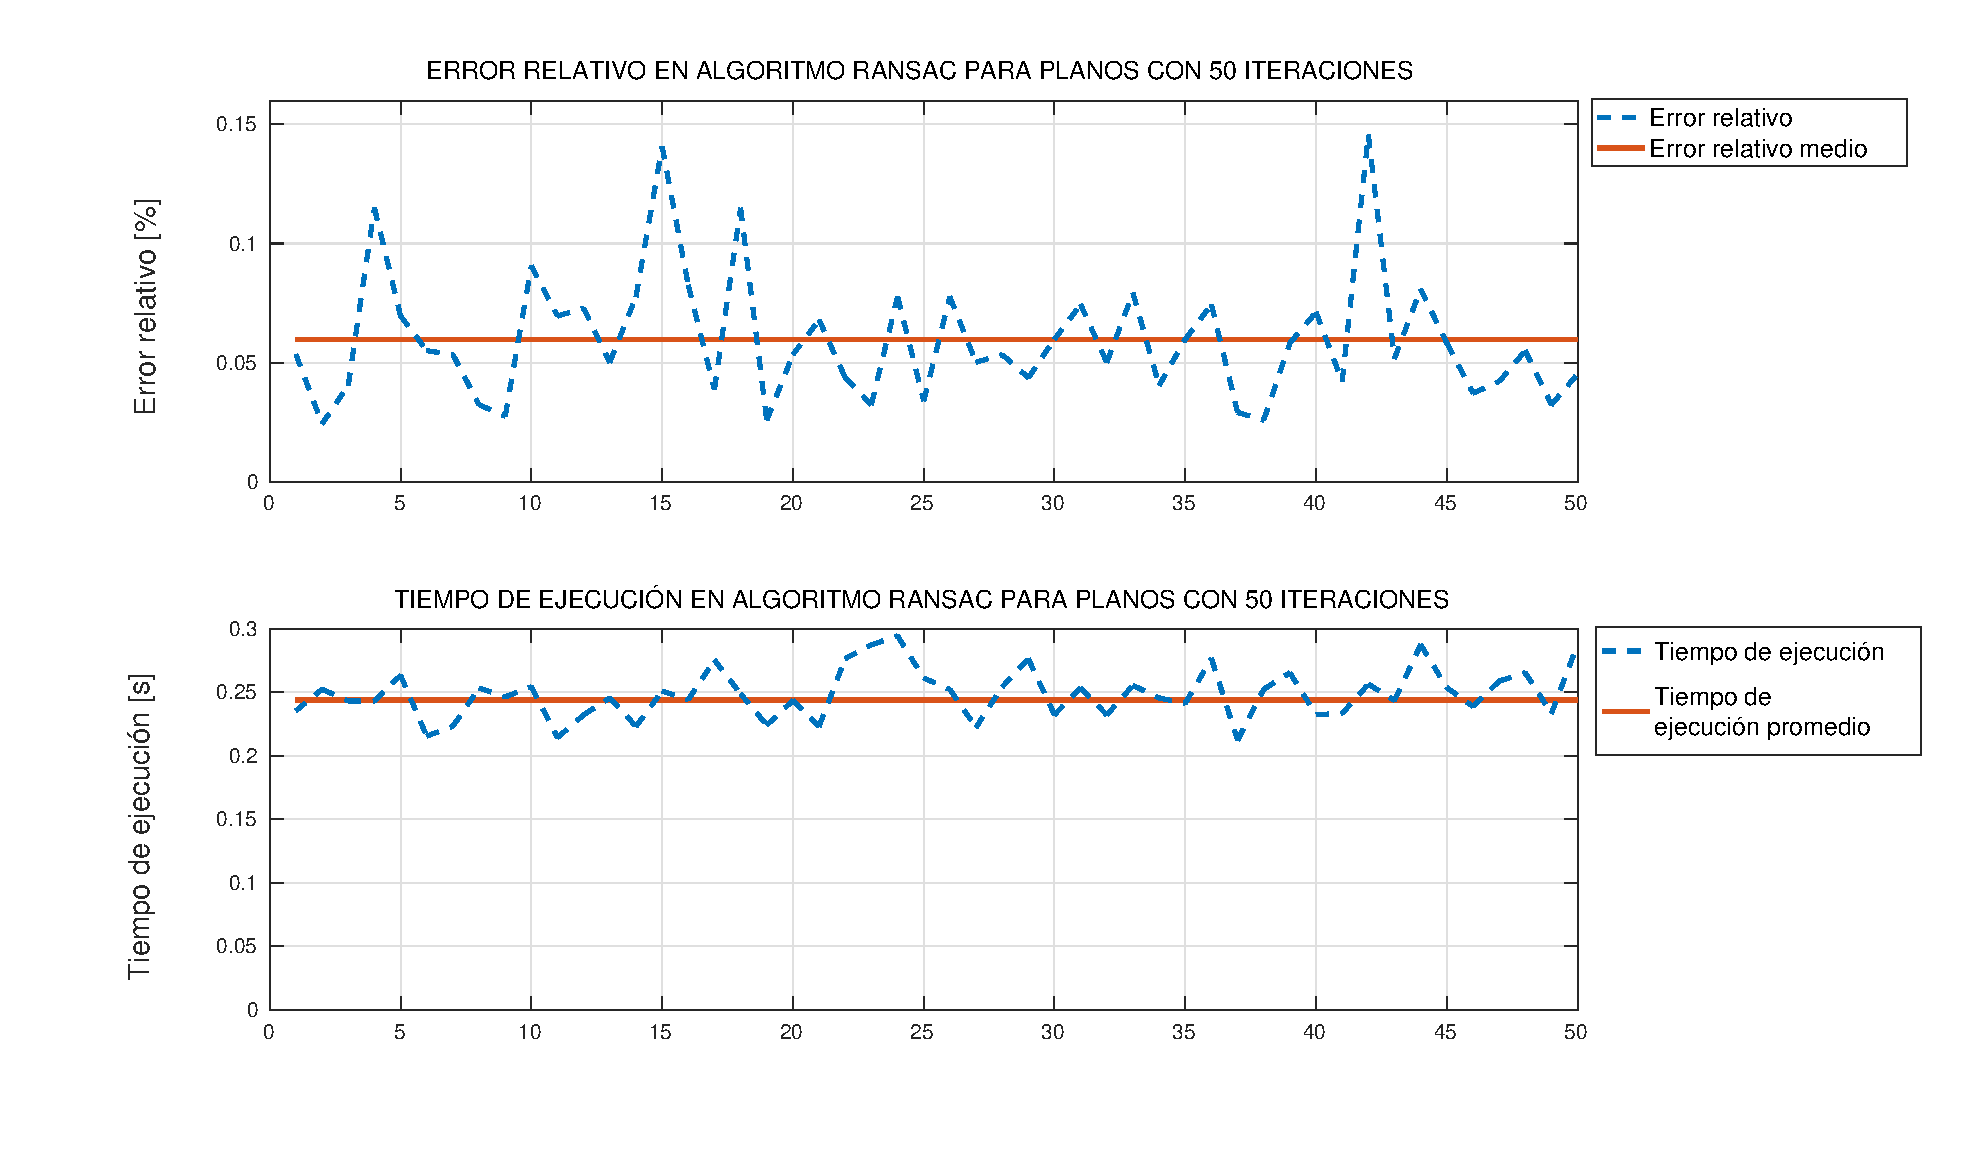
\includegraphics[width=16.0cm, height=9.0cm]{resultados/ransac_50}
		\end{minipage}
		\begin{center}
		\caption{Gráficas correspondientes al error relativo y tiempo de ejecución para el algoritmo RANSAC con 50 iteraciones.}
		\end{center}
	\end{figure}

	\begin{figure}[H]
		\begin{minipage}{18cm}
		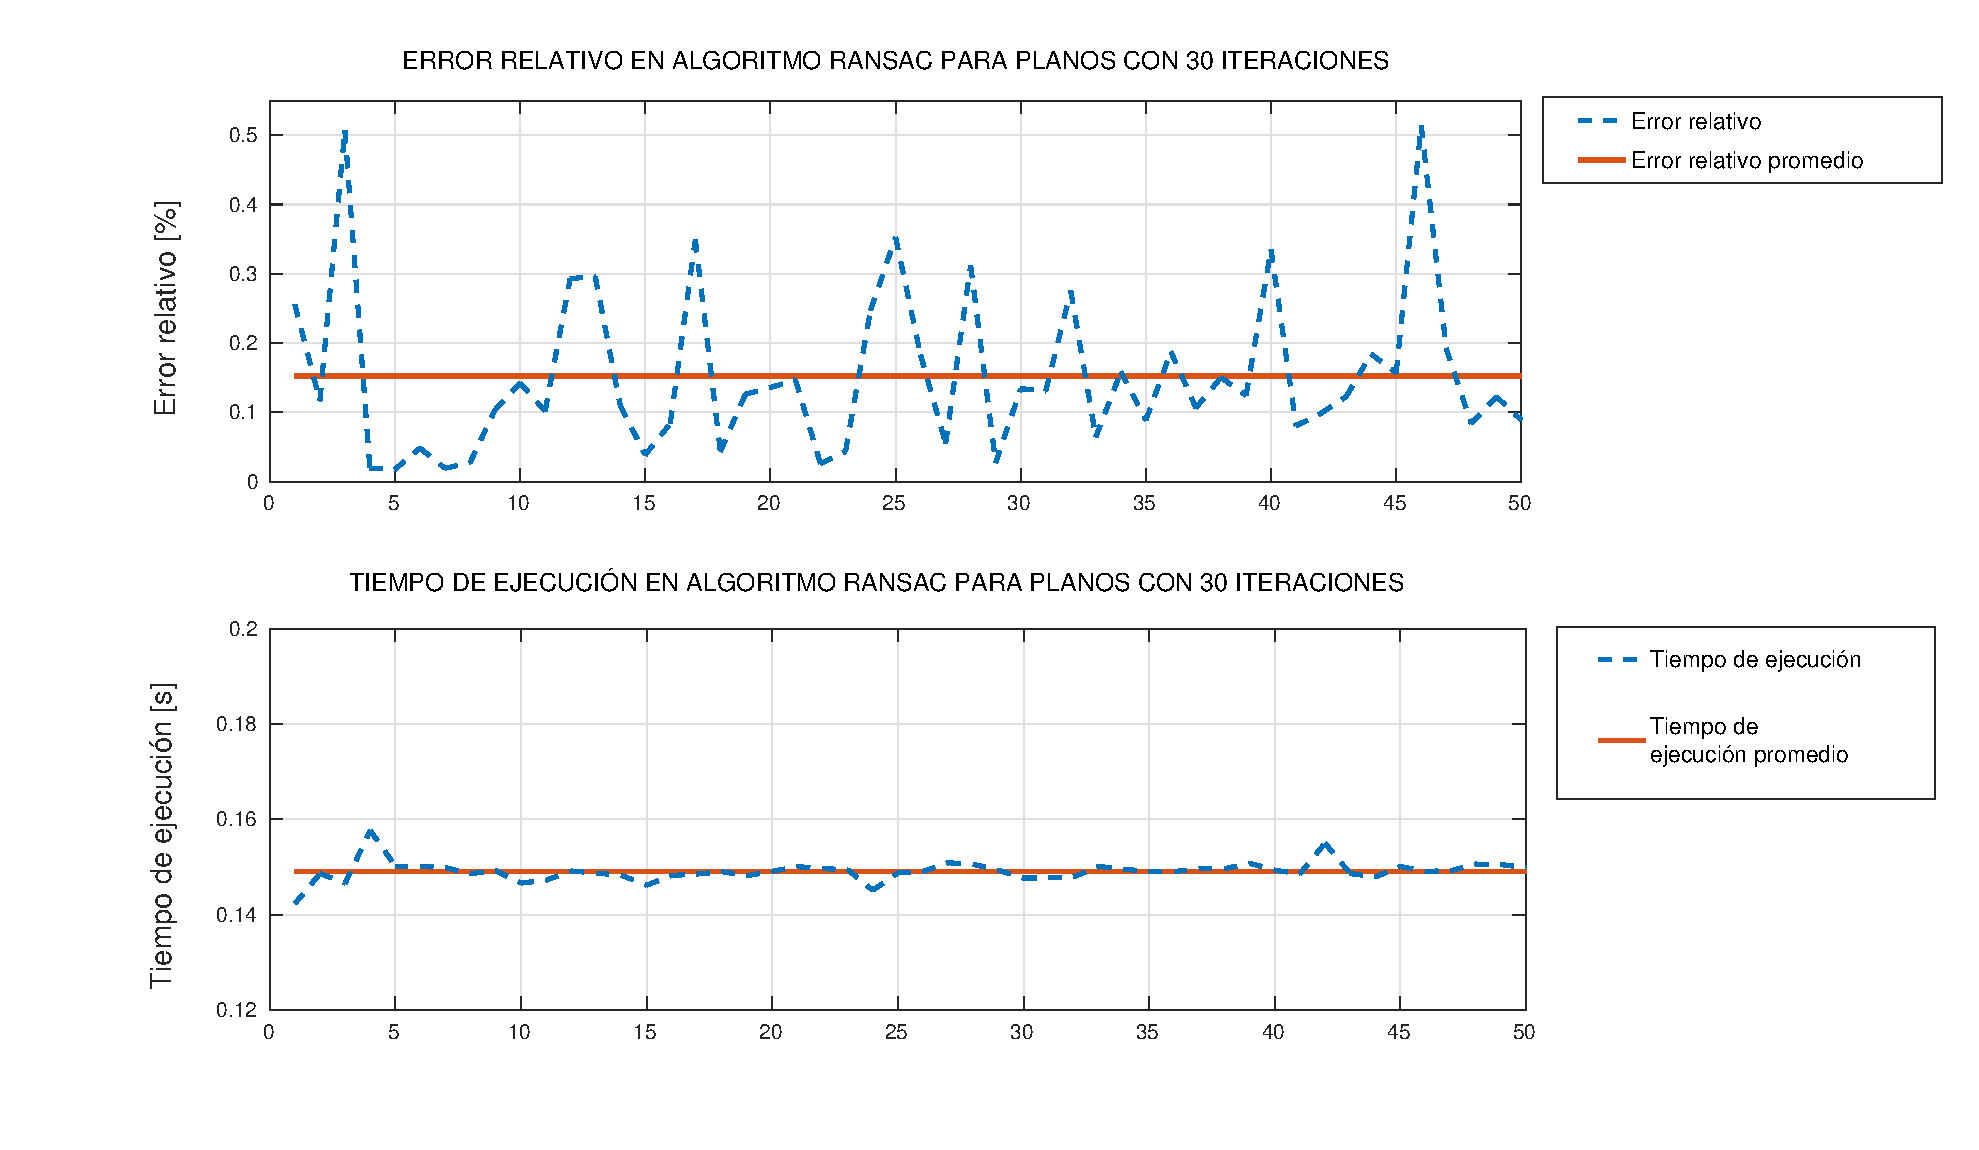
\includegraphics[width=16.0cm, height=9.0cm]{resultados/ransac_30}
		\end{minipage}
		\begin{center}
		\caption{Gráficas correspondientes al error relativo y tiempo de ejecución para el algoritmo RANSAC con 30 iteraciones.}
		\end{center}
	\end{figure}

	\begin{figure}[H]
		\begin{minipage}{18cm}
		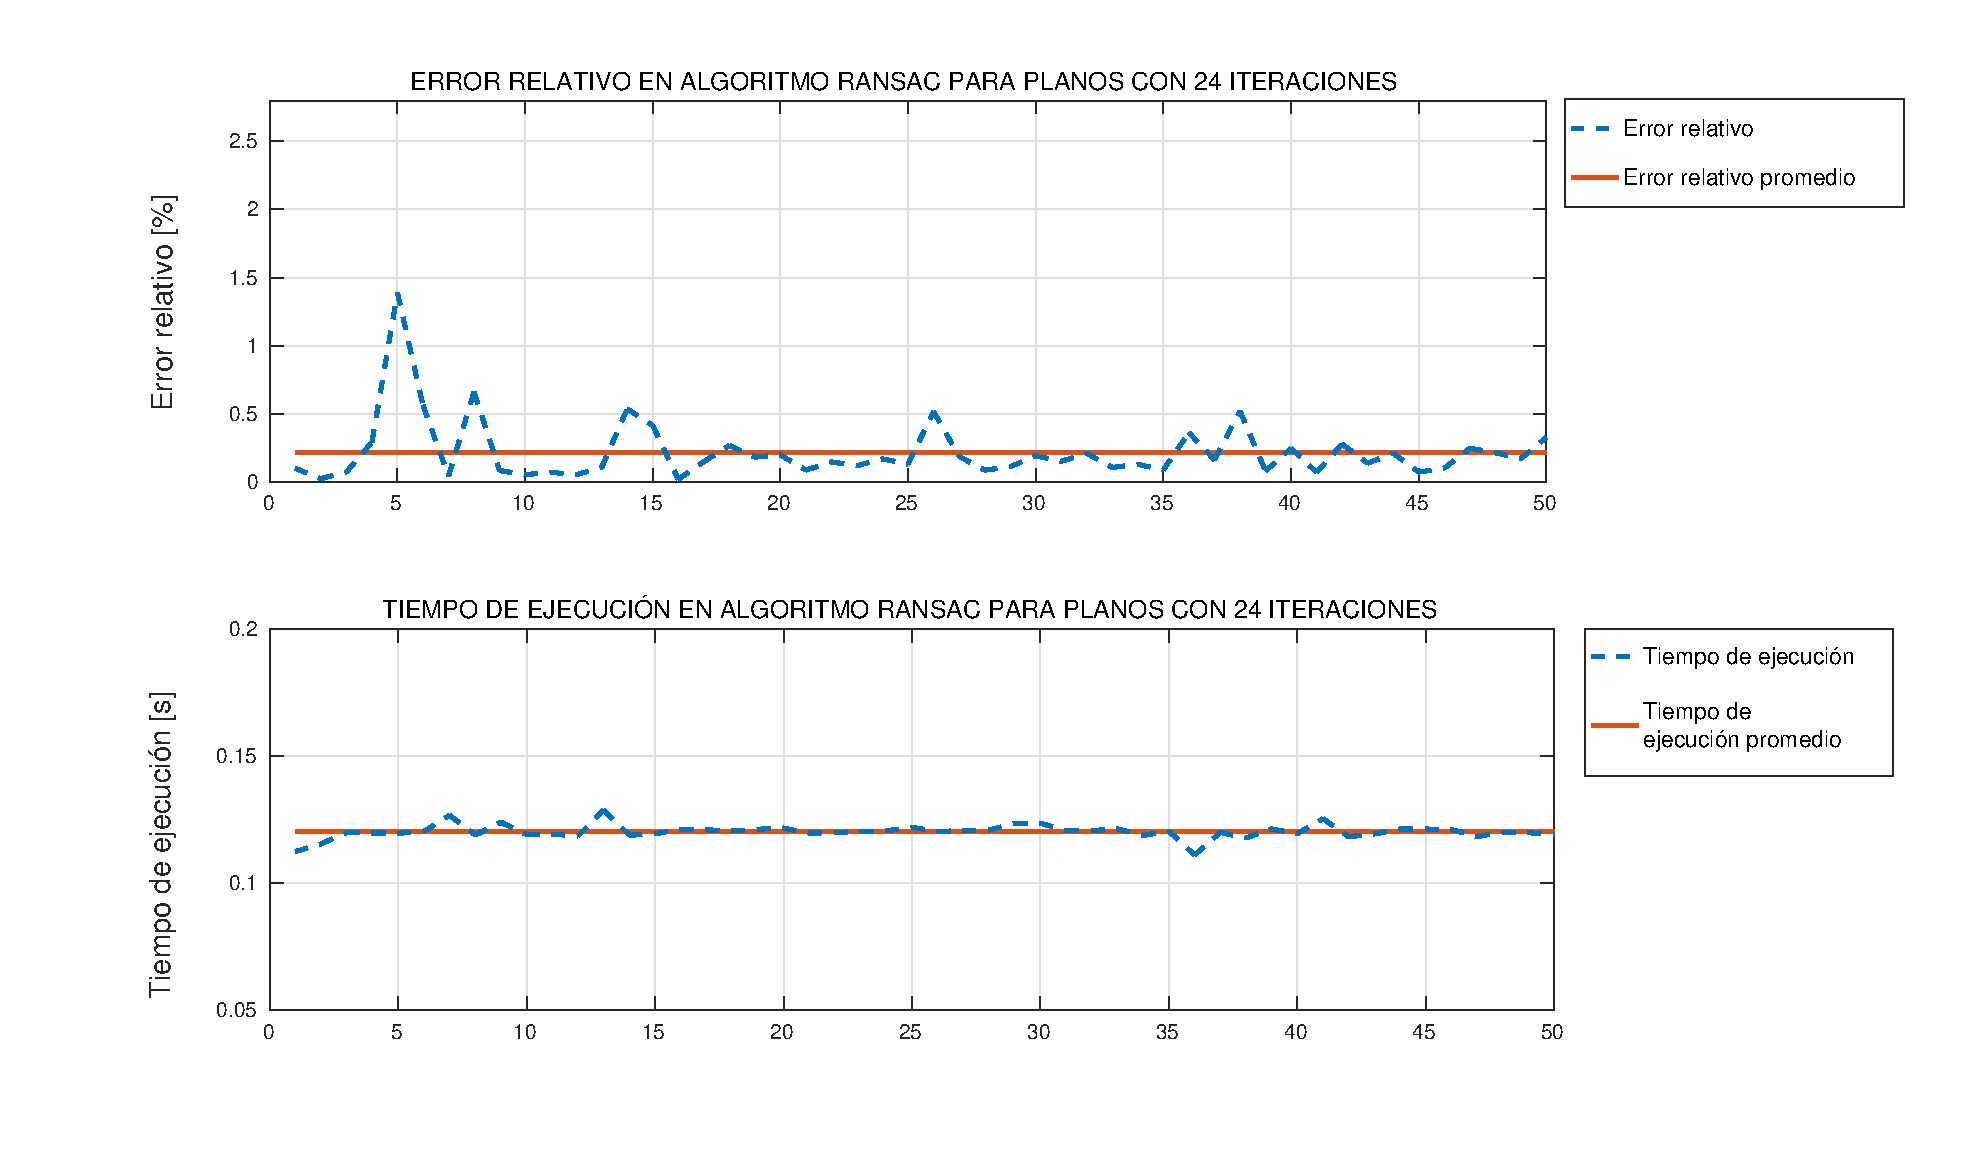
\includegraphics[width=16.0cm, height=9.0cm]{resultados/ransac_24}
		\end{minipage}
		\begin{center}
		\caption{Gráficas correspondientes al error relativo y tiempo de ejecución para el algoritmo RANSAC con 24 iteraciones.}
		\end{center}
	\end{figure}

	\begin{figure}[H]
		\begin{minipage}{18cm}	
		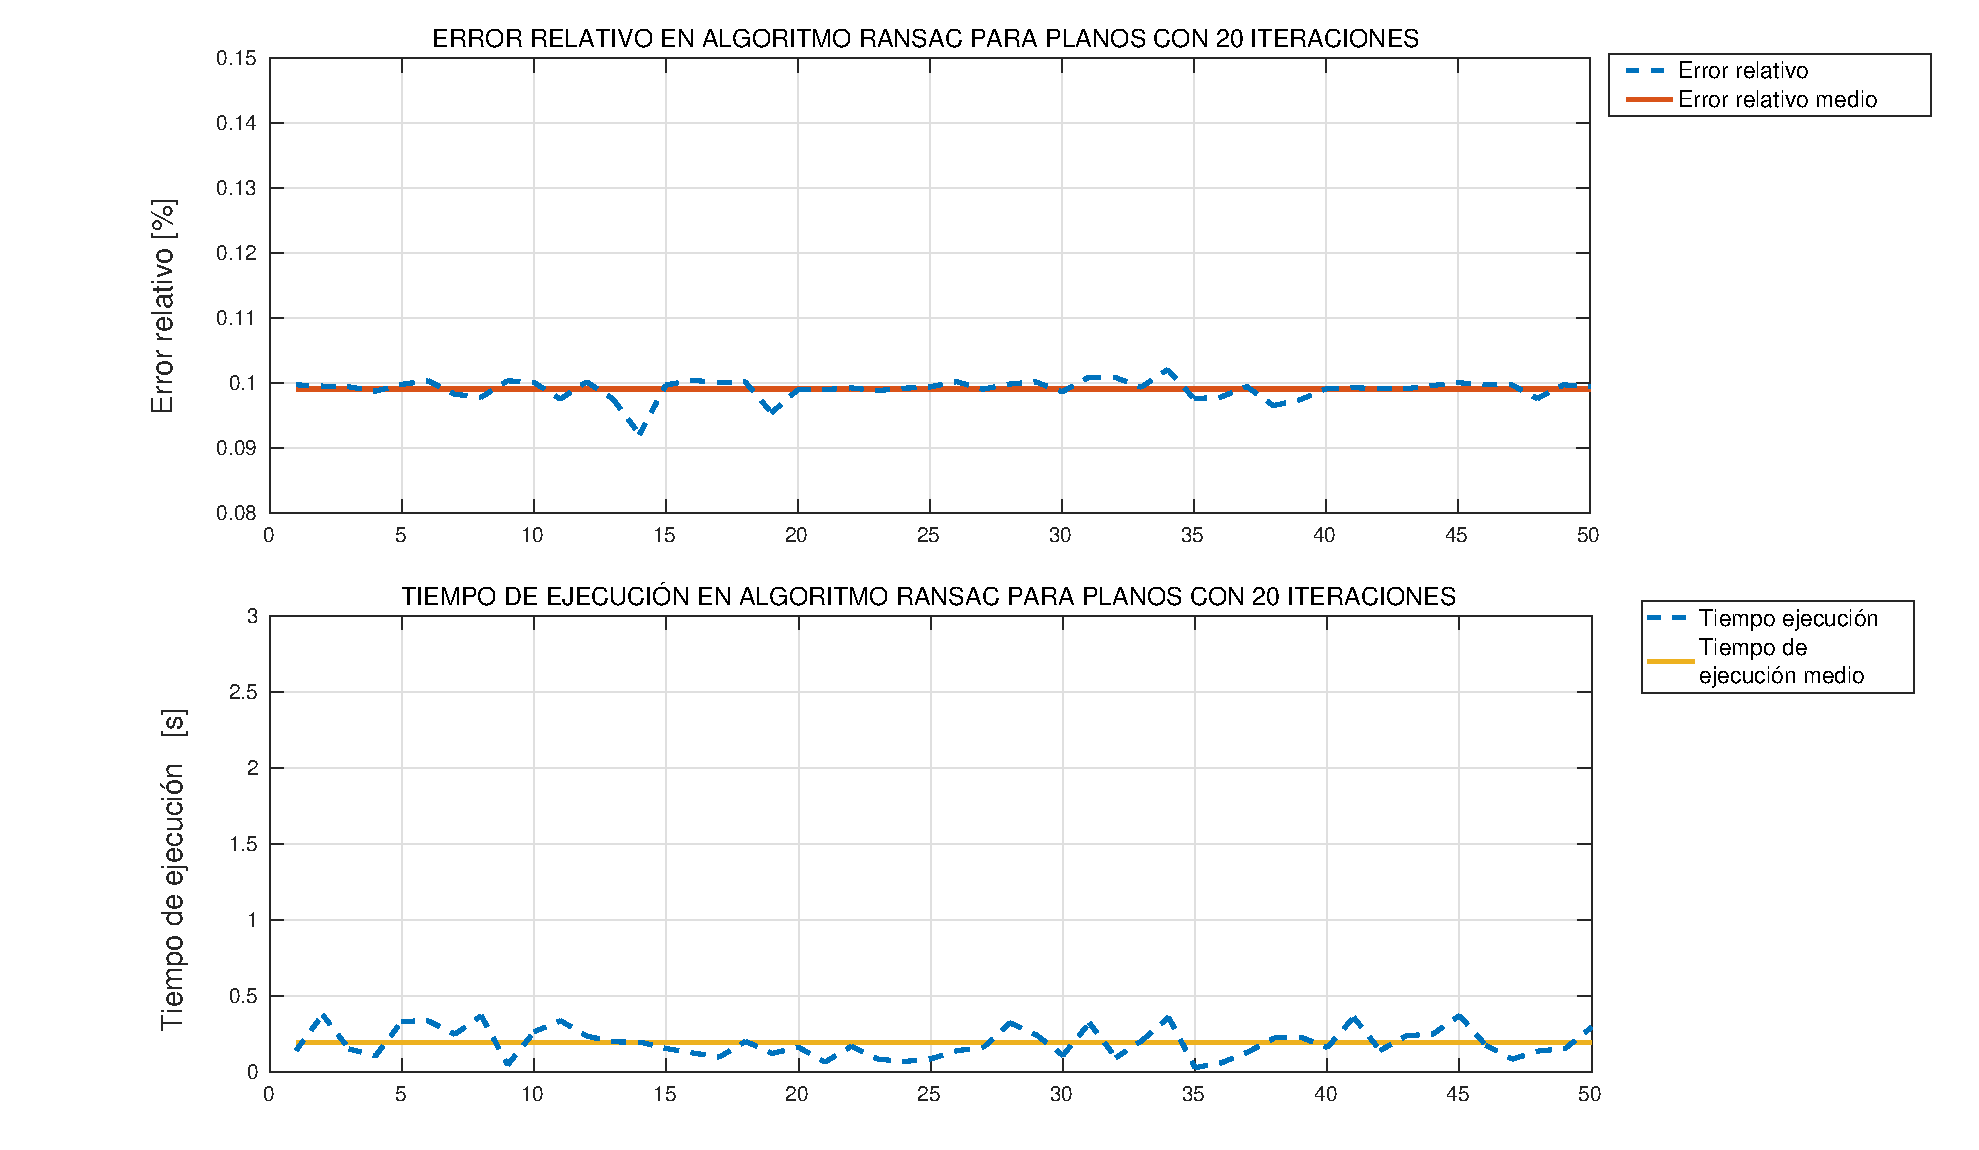
\includegraphics[width=16.0cm, height=9.0cm]{resultados/ransac_20}
		\end{minipage}
		\begin{center}
		\caption{Gráficas correspondientes al error relativo y tiempo de ejecución para el algoritmo RANSAC con 20 iteraciones.}
		\end{center}
	\end{figure}

	Una vez que se obtuvo la información parcial de cada uno de estos eventos se realizó una tabla extra que agrupa la información del tiempo de ejecución promedio y el error relativo promedio contra el número de iteraciones del algoritmo. Se obtuvo la siguiente gráfica.\\

	\begin{figure}[H]
		\begin{minipage}{18cm}
		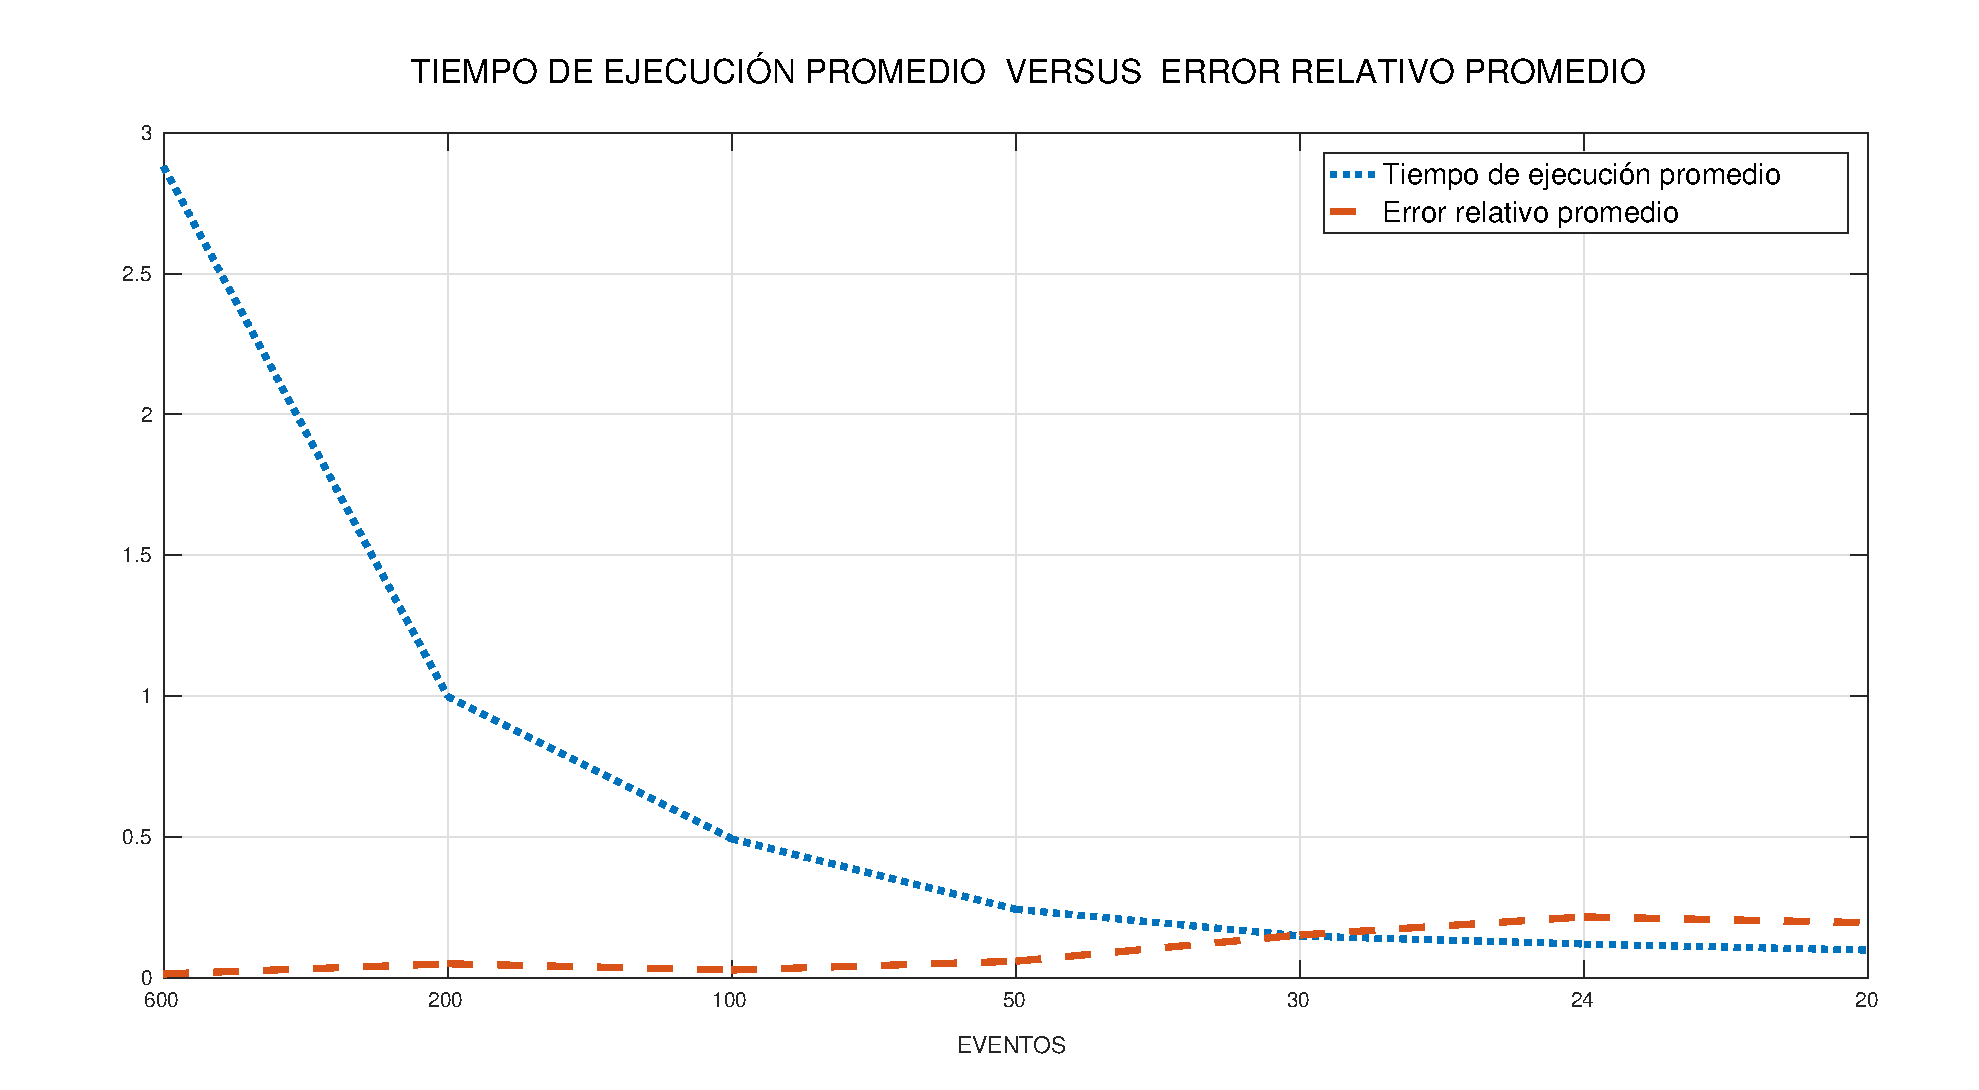
\includegraphics[width=16.0cm, height=12.0cm]{resultados/ransac_final}
		\end{minipage}

		\begin{center}
		\caption{Gráfica error relativo versus tiempo de ejecución para diferentes numeros de iteraciones.}
		\end{center}
	\end{figure}


	Como podemos observar en la tabla 4.10 el error relativo presenta un incremento conforme se disminuye el número de iteraciones en el algoritmo. El tiempo de ejecución por su parte muestra un decremento conforme número de iteraciones disminuye. Dado este comportamiento de ambos parámetros resulta difícil encontrar un punto de equilibrio entre estas dos unidades de medición. Sin embargo observamos que tanto el error relativo como el tiempo de ejecución llegan a un valor estable, a partir del cual no aumentan o disminuyen significativamente. La gráfica 4.10 nos sugiere que este punto está en un número de iteraciones entre 30 y 24.\\ 



	\subsection{Comparación exactitud y rapidez}
	Para este conjunto de pruebas se comparó el algoritmo desarrollado en el presente trabajo contra el implementado acualmente en el robot de servicio Justina. Reportado en el trabajo de tesis Jesus Cruz Navarro.\cite{cruz2016detection}\\

	Las pruebas se desarrollaron de la siguiente manera. Con la estructura de comunicación que permite ROS se implementaron dos servicios para encontrar planos: el desarrollado en este trabajo de tesis y el algortimo ya implementado. Se obtuvo la información de profundidad con el sensor RGB-D Kinect está infromación de compartió a traves de un tópico al cual ambos servicios se encontraban suscritos. De esta manera nos aseguramos de contar con la misma información en ambos algoritmos para poner a prueba la velocidad de ejecución y la precisión de algortimo.\\


	En cuanto a la medidad de precisión del algoritmo continuamos suponiendo un plano horizontal del cual conocemos su altura; por tanto podemos conocer la ecuación del plano horizontal a esa altura. Probamos el algortimo para ese modelo y observamos la cantidad de puntos que entran en ese modelo, tomando este resultado como el ideal. Posteriormente se pusieron en funcionamiento ambos algoritmos midiendo la cantidad de puntos en los modelos obtenidos y comparadolos con el número de puntos ideal. Este evento se iteró una cantidad aproximada de 80 veces.\\


	Posteriormente calculamos el error relativo entre el modelo ideal y cada uno de los algoritmos. Como se muestran en la gráfica siguiente.\\


	La tabla \ref{t_result:1} resume los resultados obtenidos durante las pruebas.\\

	\begin{table}[h!]
	\centering 
	\begin{tabular}{ |p{6.5cm}||p{2.1cm}|p{2.1cm}|  }
	 \hline
	 \multicolumn{3}{|c|}{ Resultados algoritmo RANSAC } \\
	 \hline
	 \multicolumn{3}{|c|}{ Número de iteraciones: 1000}\\
	 \hline
	 \multicolumn{3}{|c|}{ Distancia miníma al modelo: 0.02[m]}\\
	 \hline
	                               &  Anterior     &	Actual \\
	 \hline
	 Tiempo promedio de ejecución  &  96.24[ms]    &   701.5[ms]\\
	 \hline
	 Error relativo promedio       &  39.95        &    8.78\\
	 \hline
	\end{tabular}
	\caption{Comparación de resultados de RANSAC para planos.}
	\label{t_result:1}
	\end{table}


	Con la información de que se ha reflejado en la tabla \ref{t_result:1} se puede deducir que la nueva implementación del algoritmo RANSAC con 1000 iteraciones y una distancia miníma al modelo de 0.02[m] es más lenta pero con menor error relativo. La diferencia de 605[ms] puede llegar a ser significativa si se requiere ejecutar el algoritmo iterativamente, sin embargo el común de las pruebas en ambientes del hogar no suelen requerir este tipo de acciones.\\  





\newpage
%%%%%%%%%%%%%%%%%%%%%%%%%%%%%%%%%%%%%%%%%%%%%%%%%%%%%%%%%%%%%%%%%%%%
%%%%%%%%%     CARACTERISTICAS OBJETOS          %%%%%%%%%%%%%%%%%%%%%
	\section{Extracción de objetos y sus características}
	En lo que respecta a la extracción de objetos y sus características se procedió a realizar una caracterización de la misma. Para ello se realizaron un total de 100 eventos para cada uno de los 5 objetos diferentes: un control para videojuegos de forma irregular, una caja de cereal, un envase de jugo, un envase de bebida láctea y una barra de chocolate. Como información de interés se compararón las medidas de altura de los objetos. Puesto que el algoritmo previo tambien hacía una estímación de la altura de los objetos se compararon los resultados de ambos algoritmos. Como elementos de medida signiticativos se tomaron medida de tendencia central (valor esperado del dentroide) y como medida de dispersión se tomó la varianza. A continuación se presentan los resultados obtenidos de las mediciones realizadas.\\

	\begin{figure}[H]
		\centering
		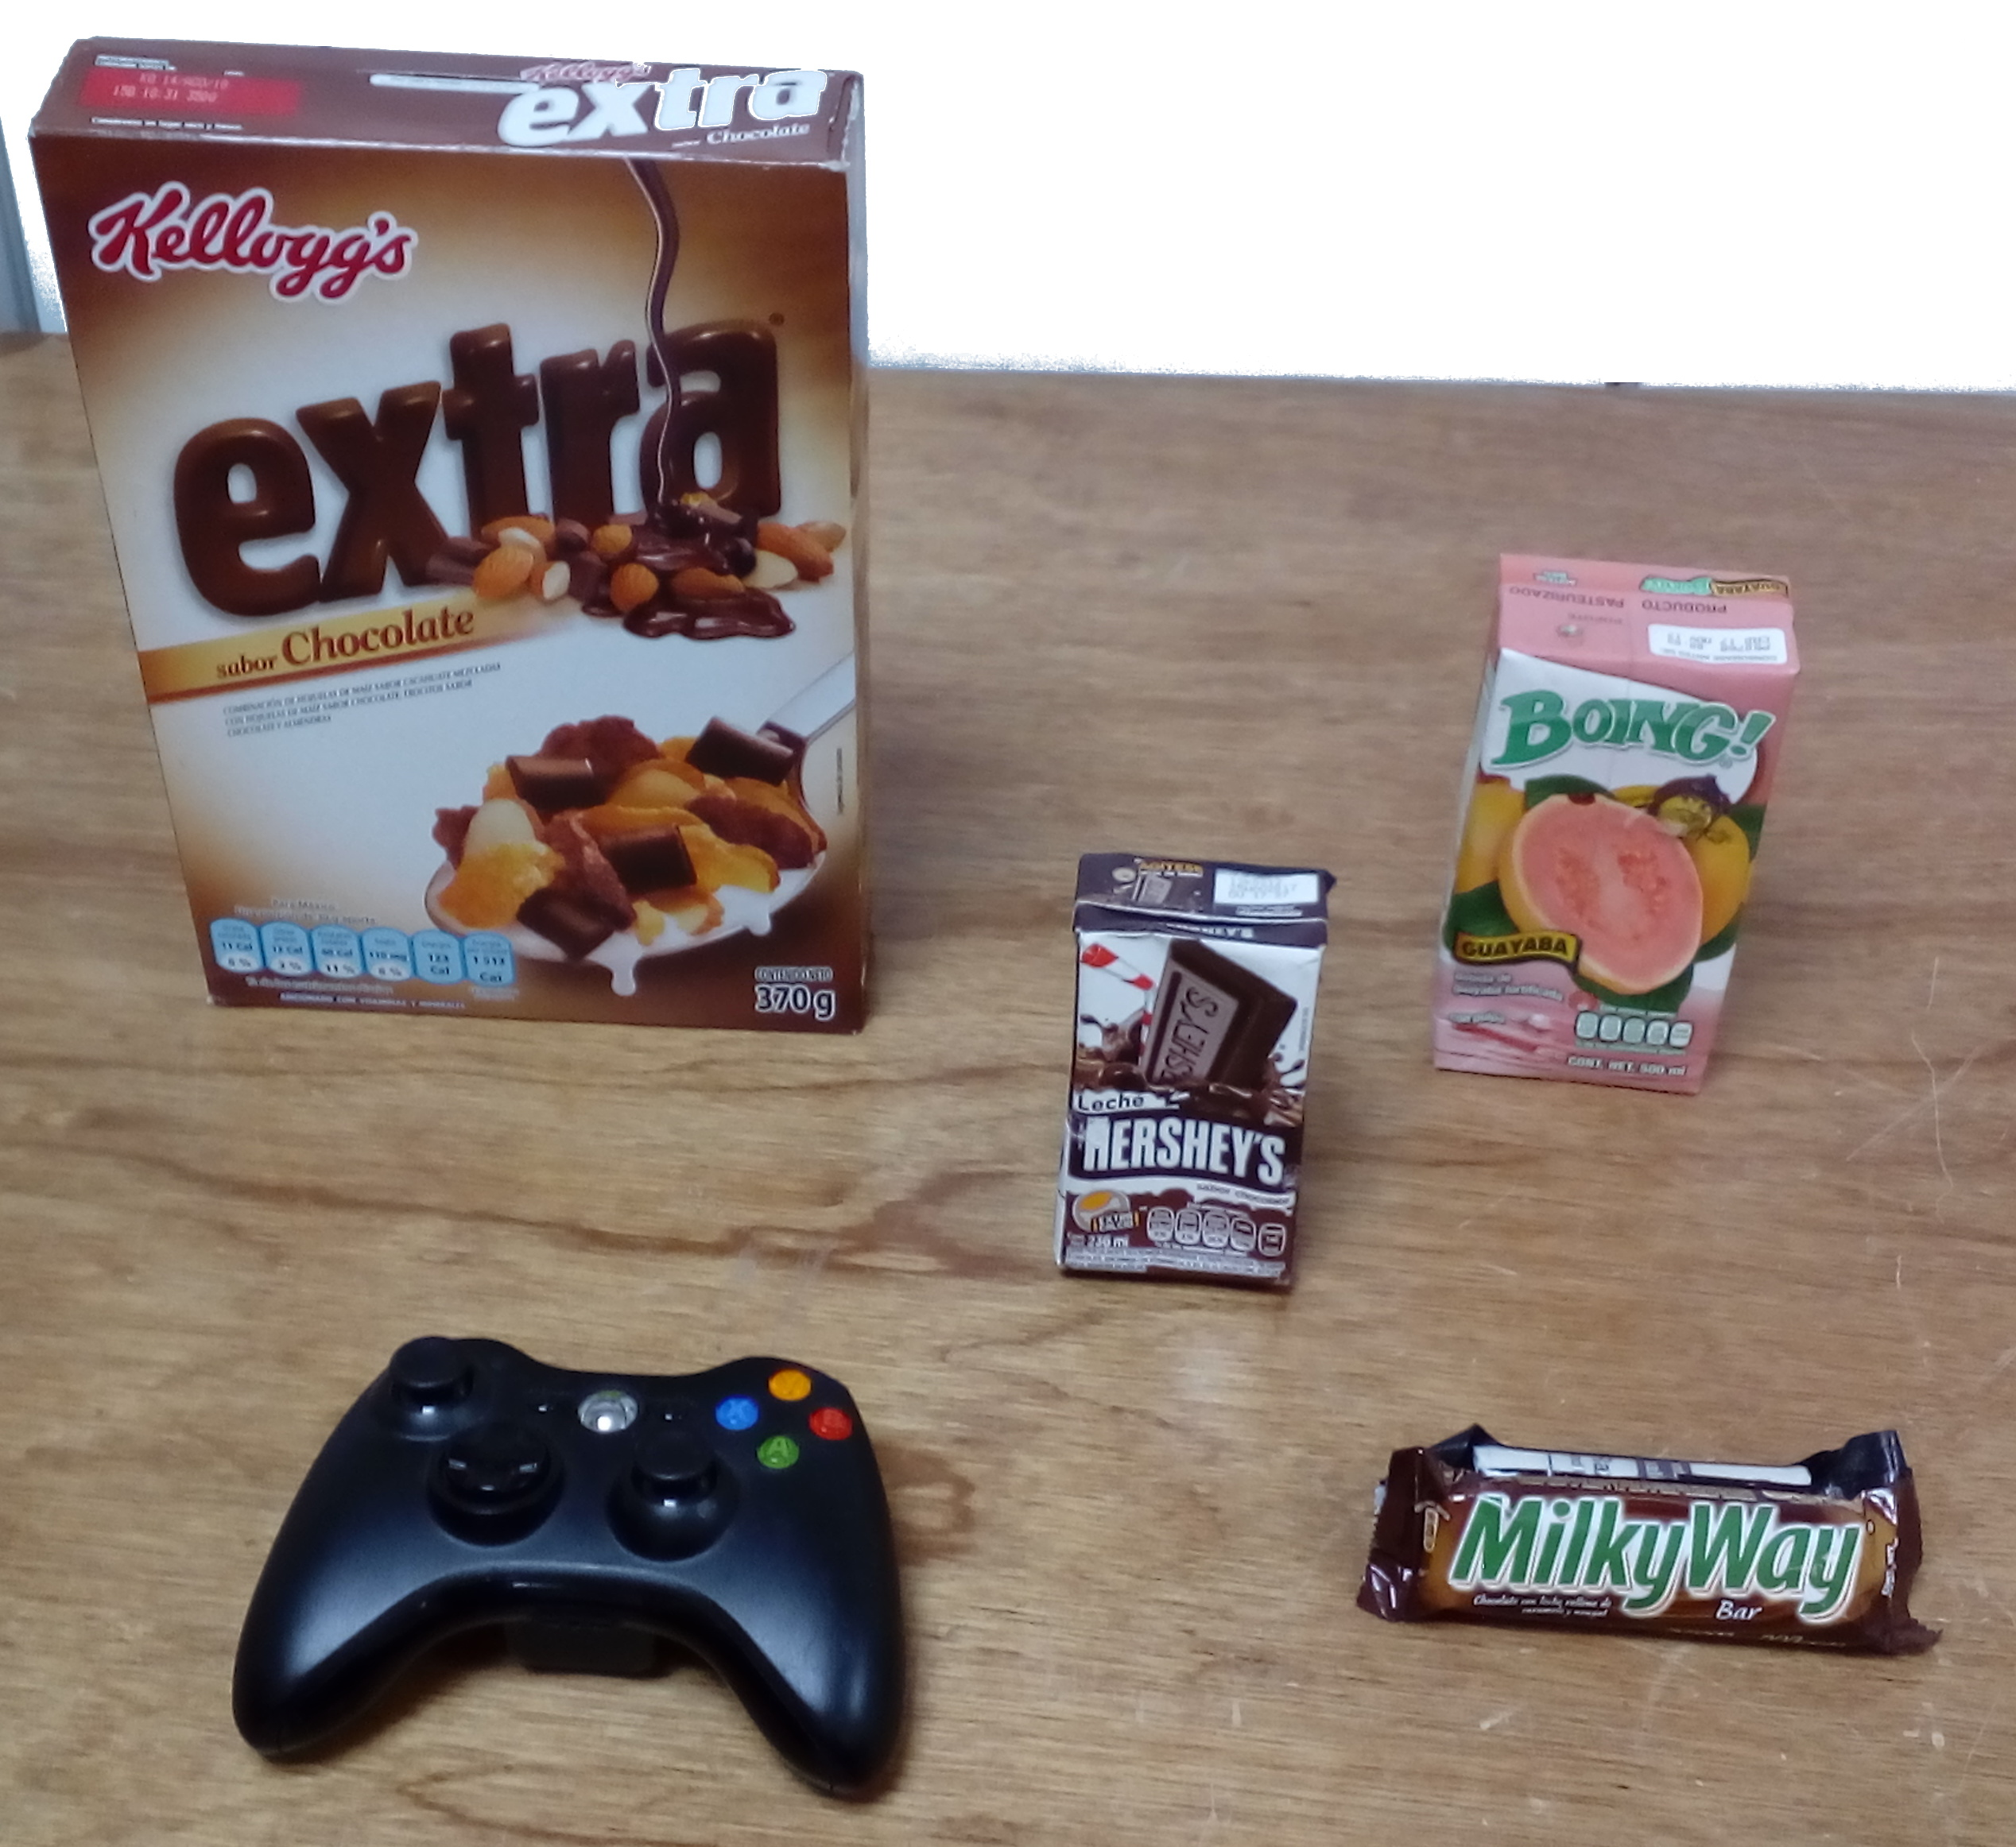
\includegraphics[scale=0.06]{objs_real/objects_2.jpg}	
		\caption{Fotografia de los objetos utilizados en las pruebas de cálculo de alturas y de manipulación de objetos.}
		\label{fig:objectsComplete}
	\end{figure}


	\subsection{Estímación de alturas}

	\begin{figure}[H]
		\begin{subfigure}[h]{.30\textwidth}
		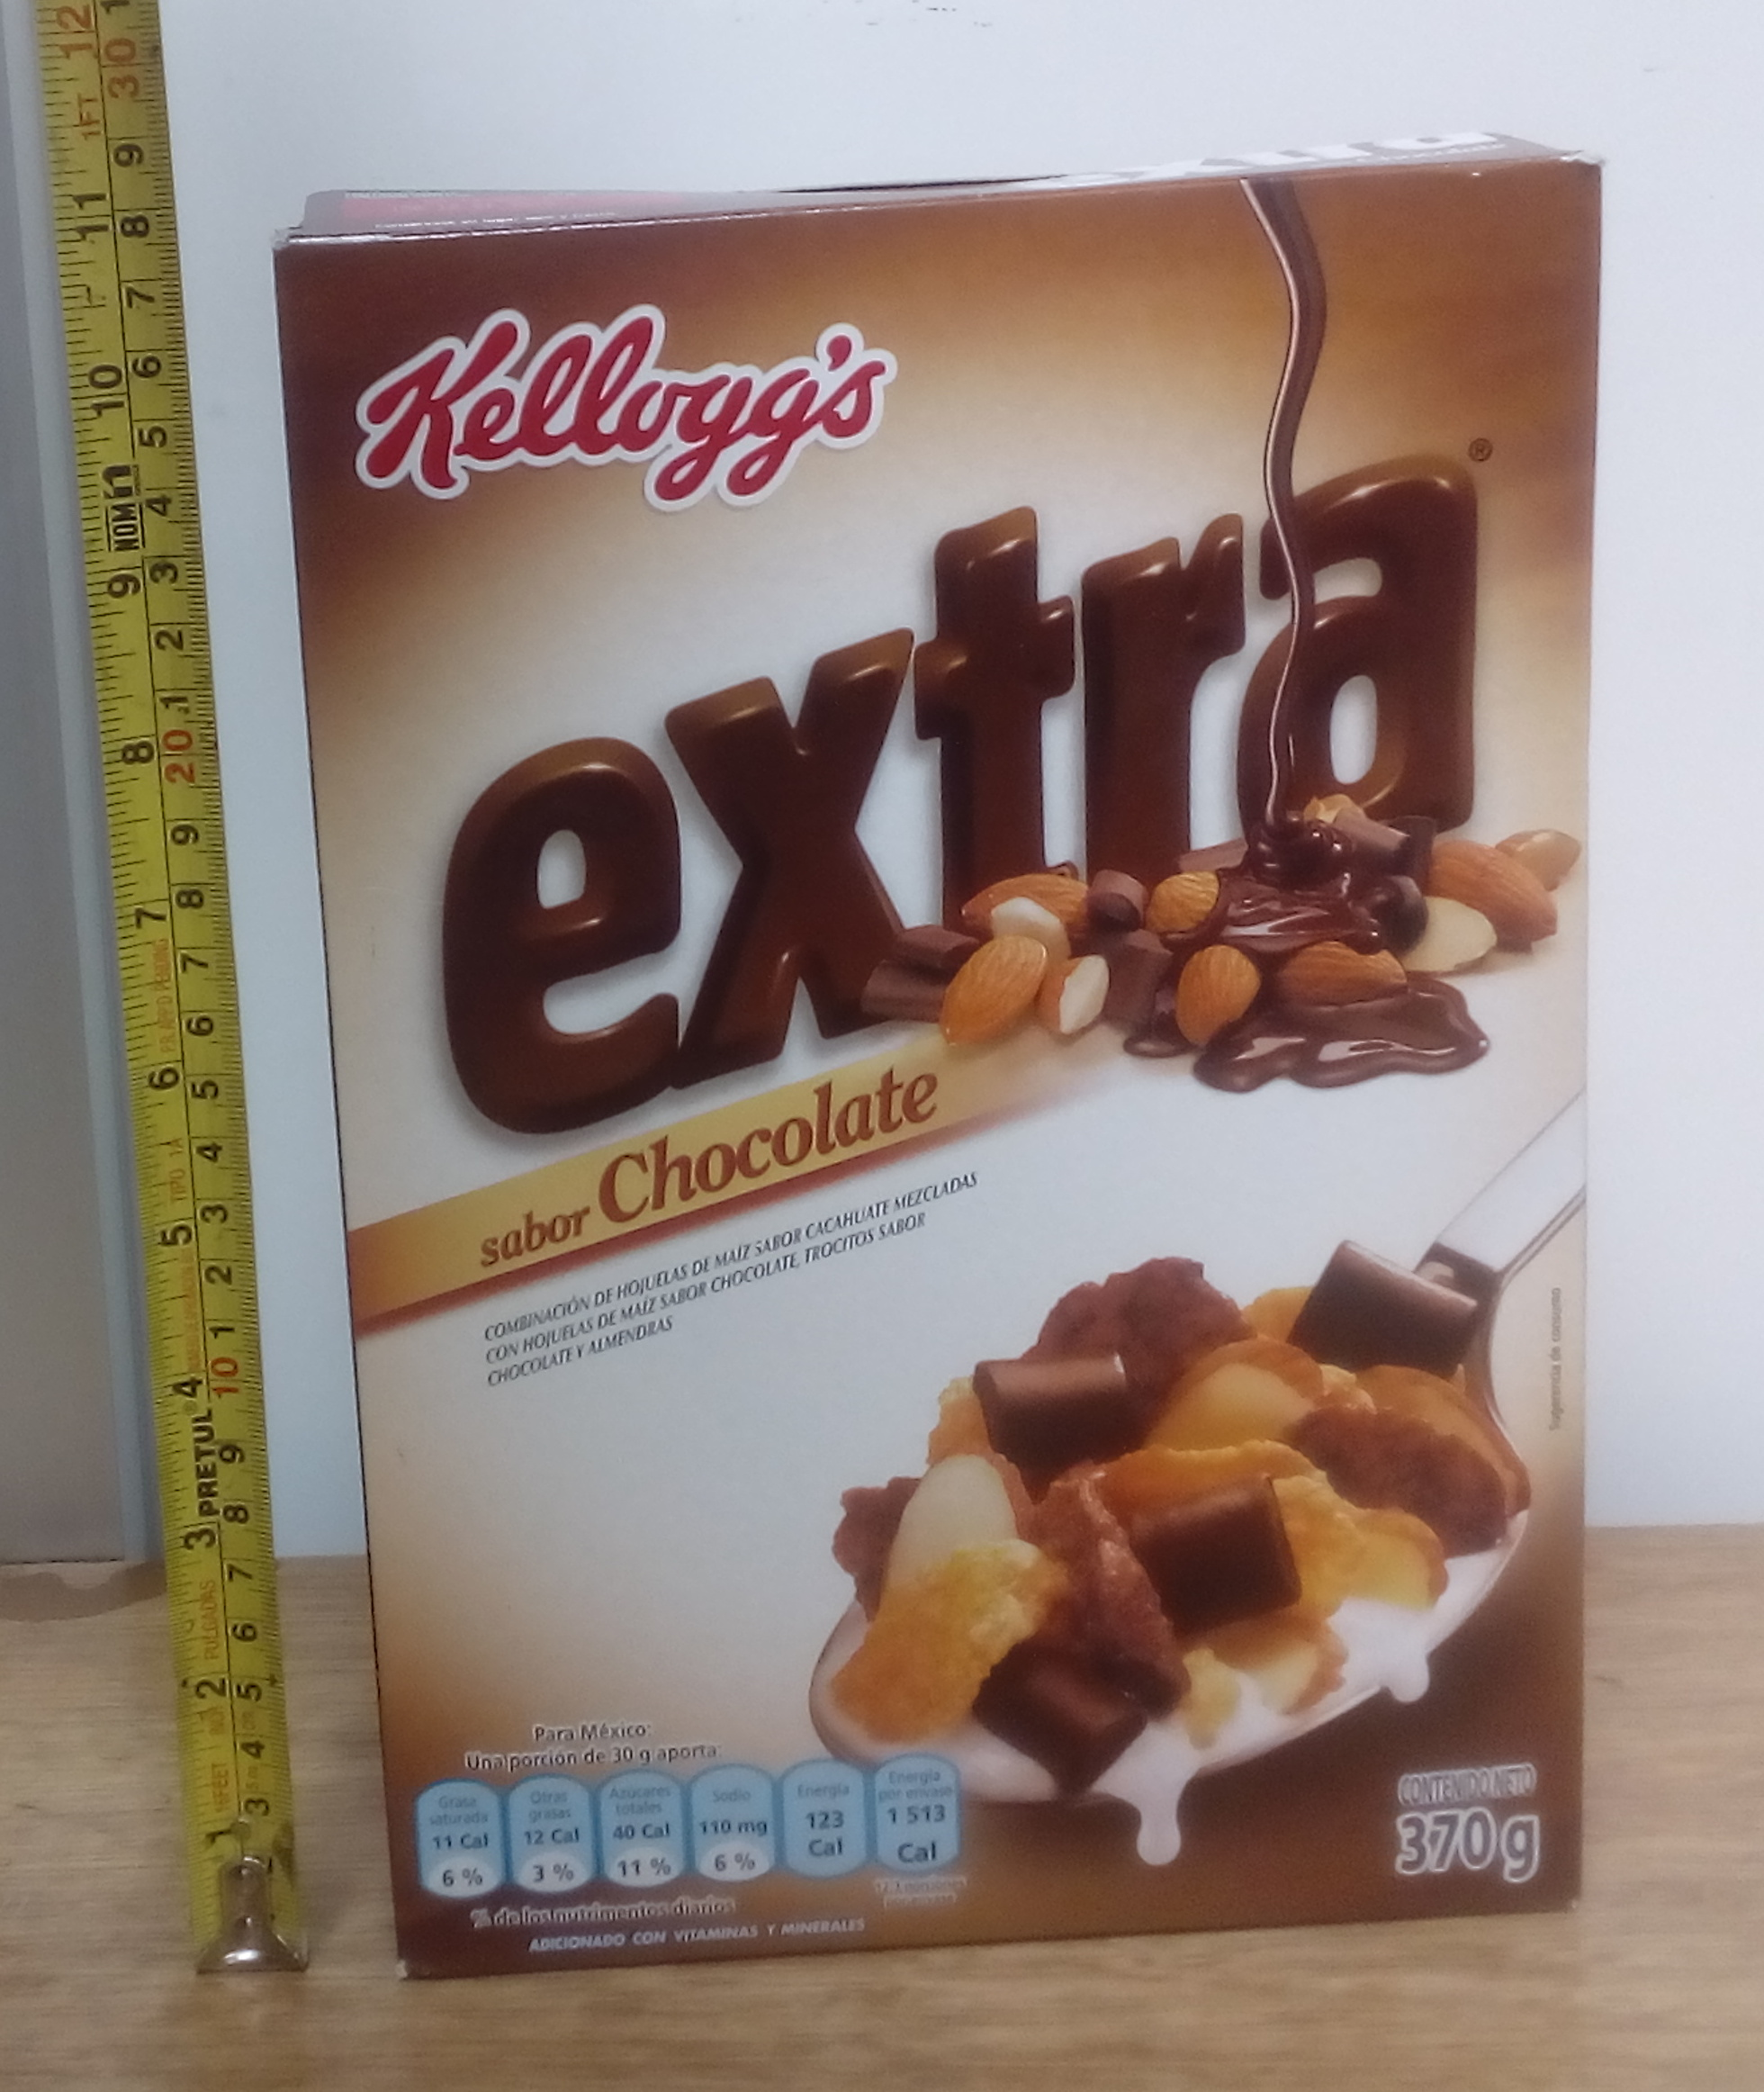
\includegraphics[scale=0.05]{objs_real/cerealBoxHeight.jpg}	
		\end{subfigure}%
		\begin{subfigure}[h]{.5\textwidth}
		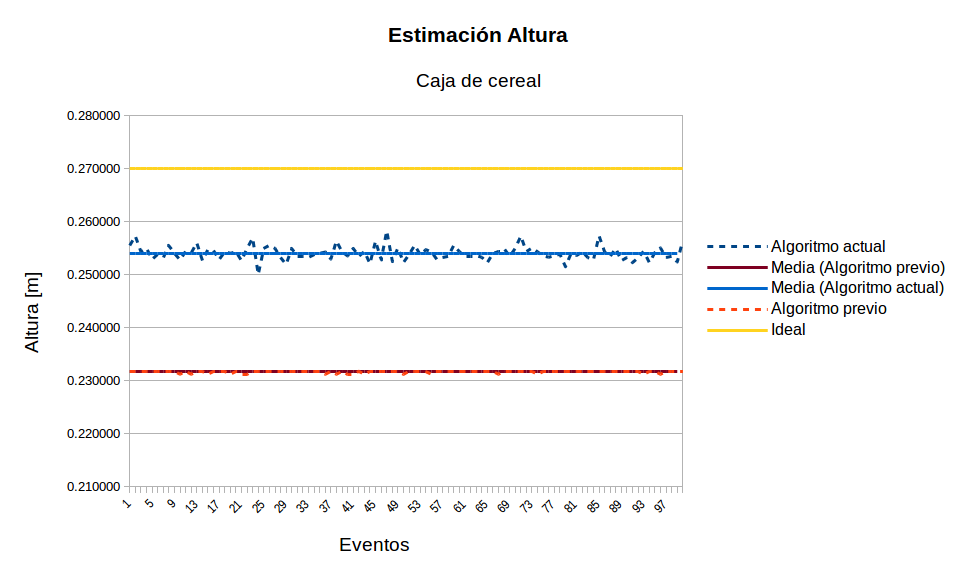
\includegraphics[scale=0.45]{resultados/cerealAltura_media.png}	
		\end{subfigure}
		\caption{Gráficas de estímaciones de alturas para una caja de cereal. La altura real del objeto (amarillo), la altura estímada con el algoritmo previo (rojo) y la estimación actual (azul).}
		\label{fig:mesh1}
	\end{figure}

	\begin{figure}[H]
		\begin{subfigure}[h]{.30\textwidth}
		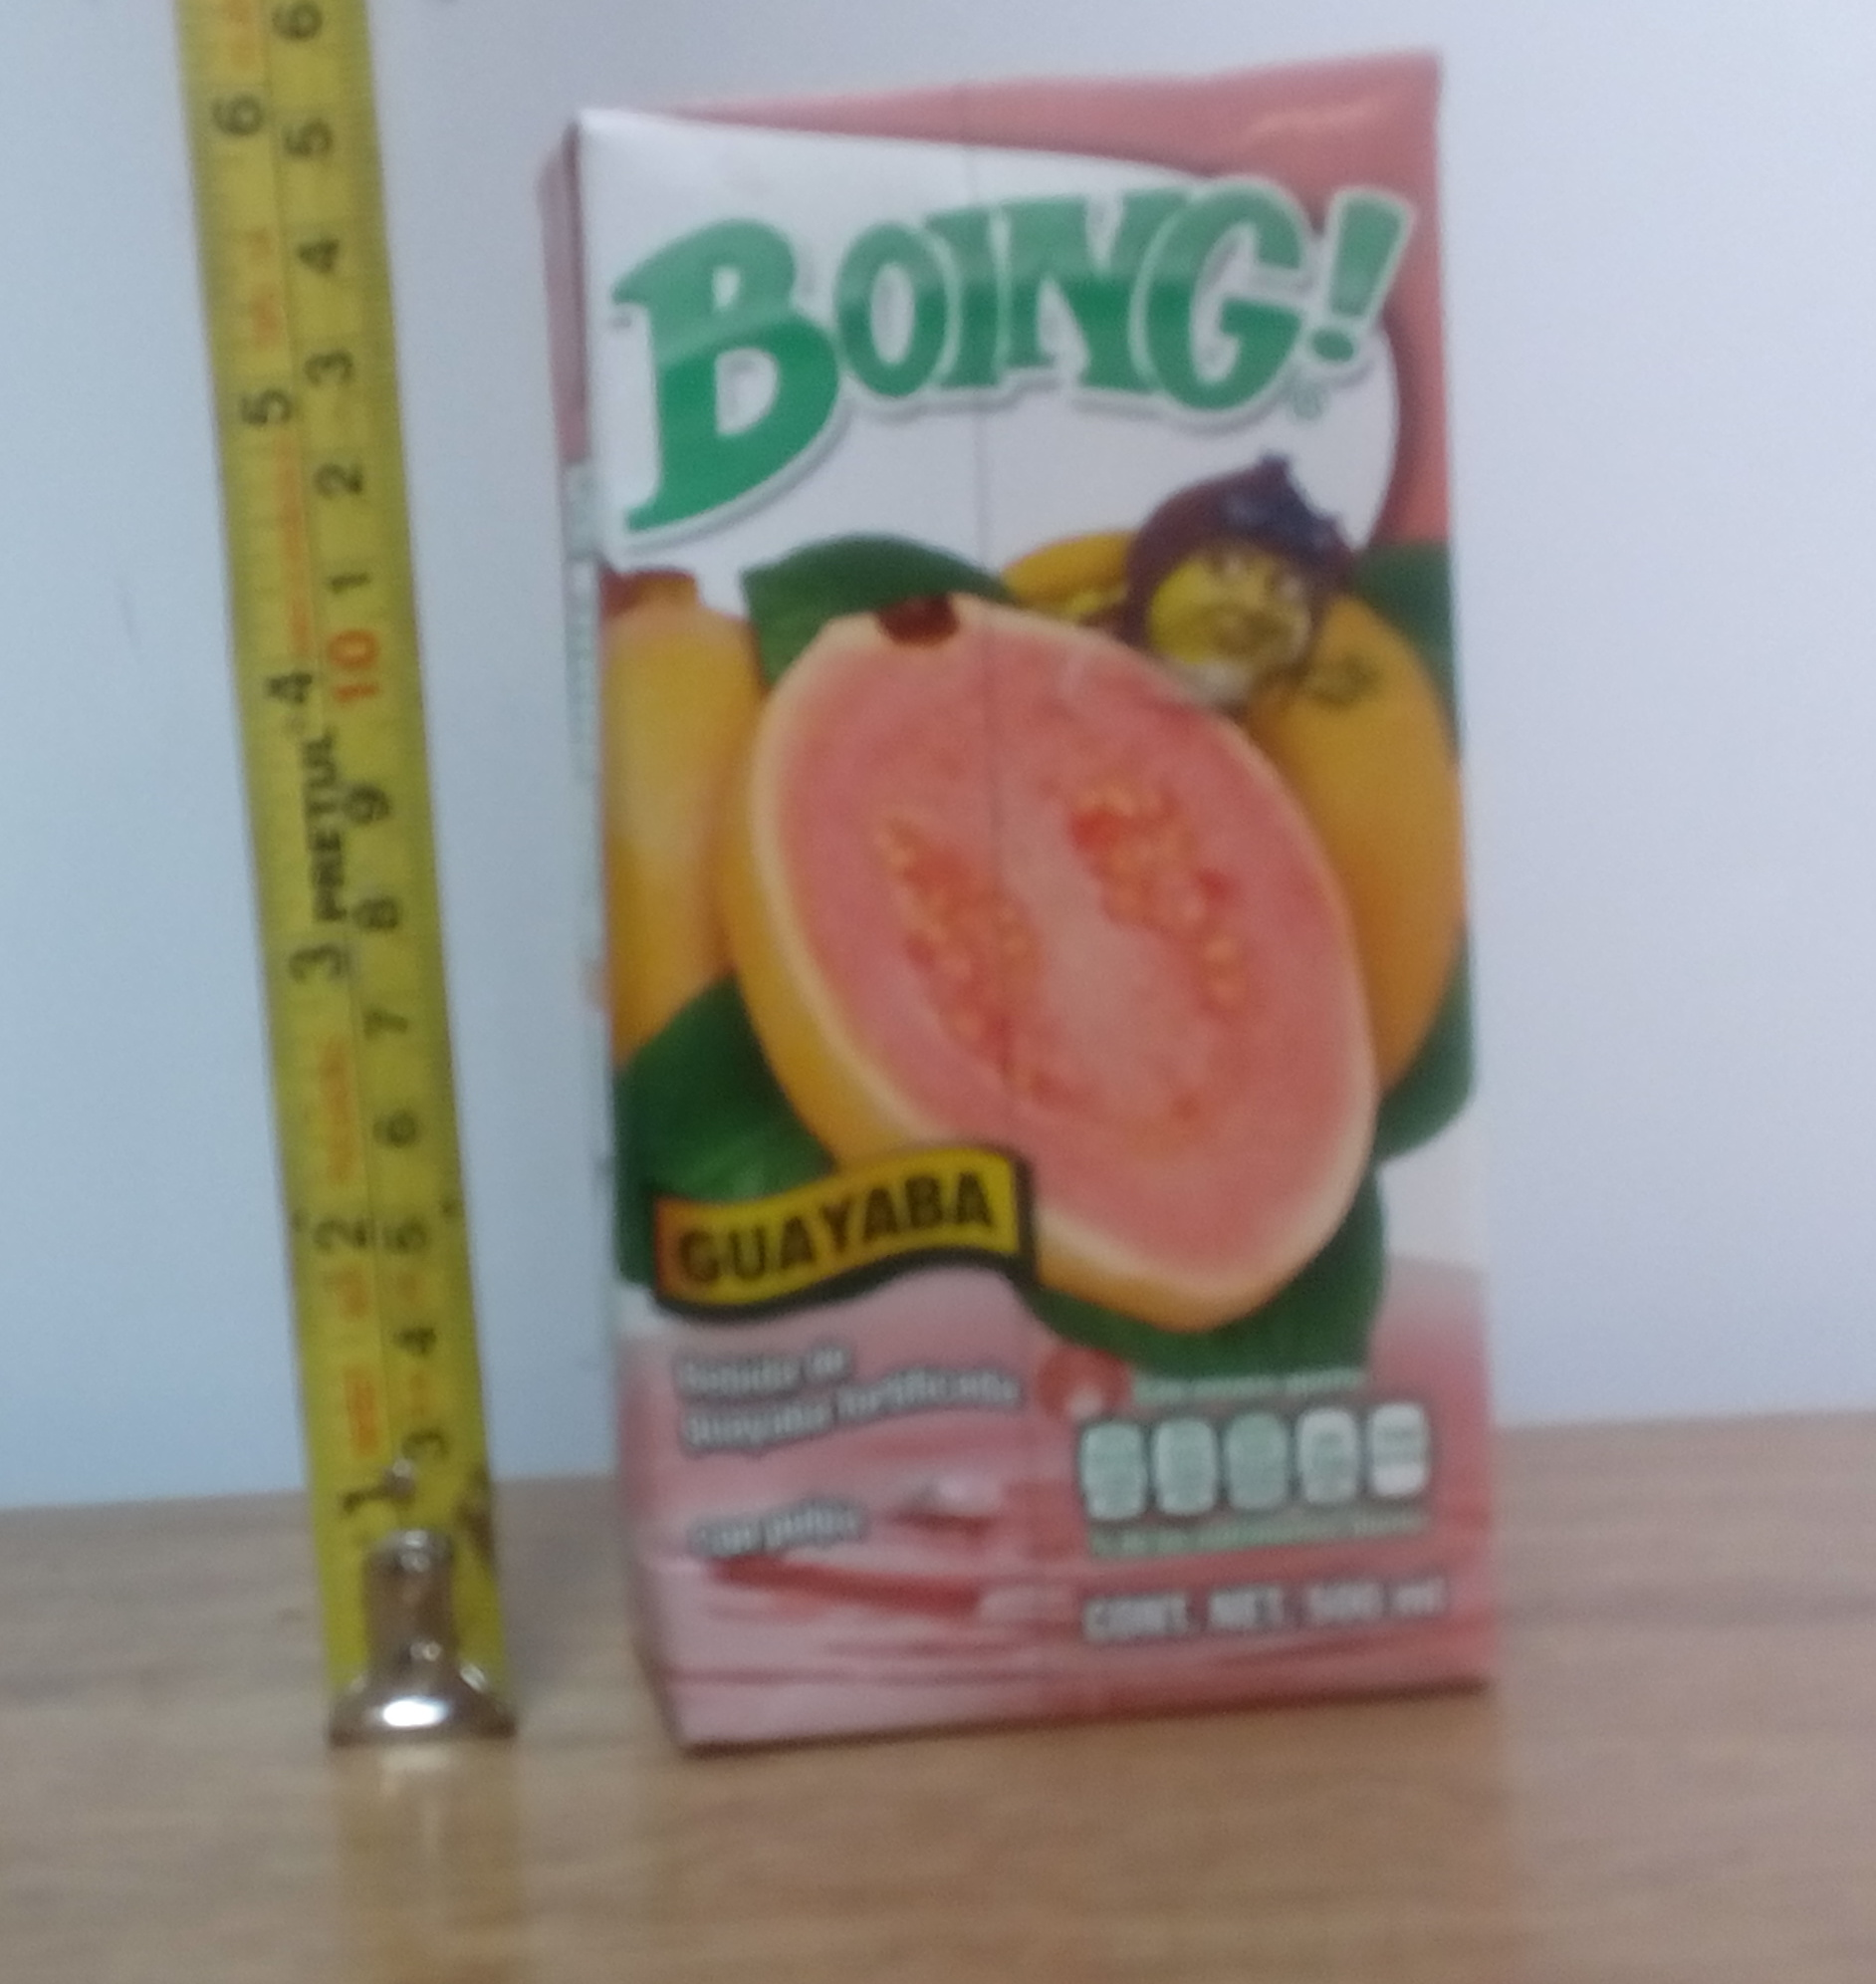
\includegraphics[scale=0.05]{objs_real/jugoHeight.jpg}	
		\end{subfigure}%
		\begin{subfigure}[h]{.5\textwidth}
		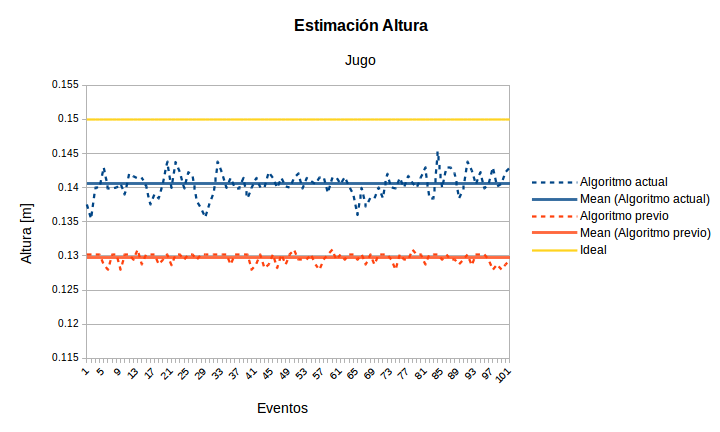
\includegraphics[scale=0.45]{resultados/jugoAltura_media.png}	
		\end{subfigure}
		\caption{Gráficas de estímaciones de alturas para un envase de jugo. La altura real del objeto (amarillo), la altura estímada con el algoritmo previo (rojo) y la estimación actual (azul).}
		\label{fig:mesh1}
	\end{figure}

	\begin{figure}[H]
		\begin{subfigure}[h]{.30\textwidth}
		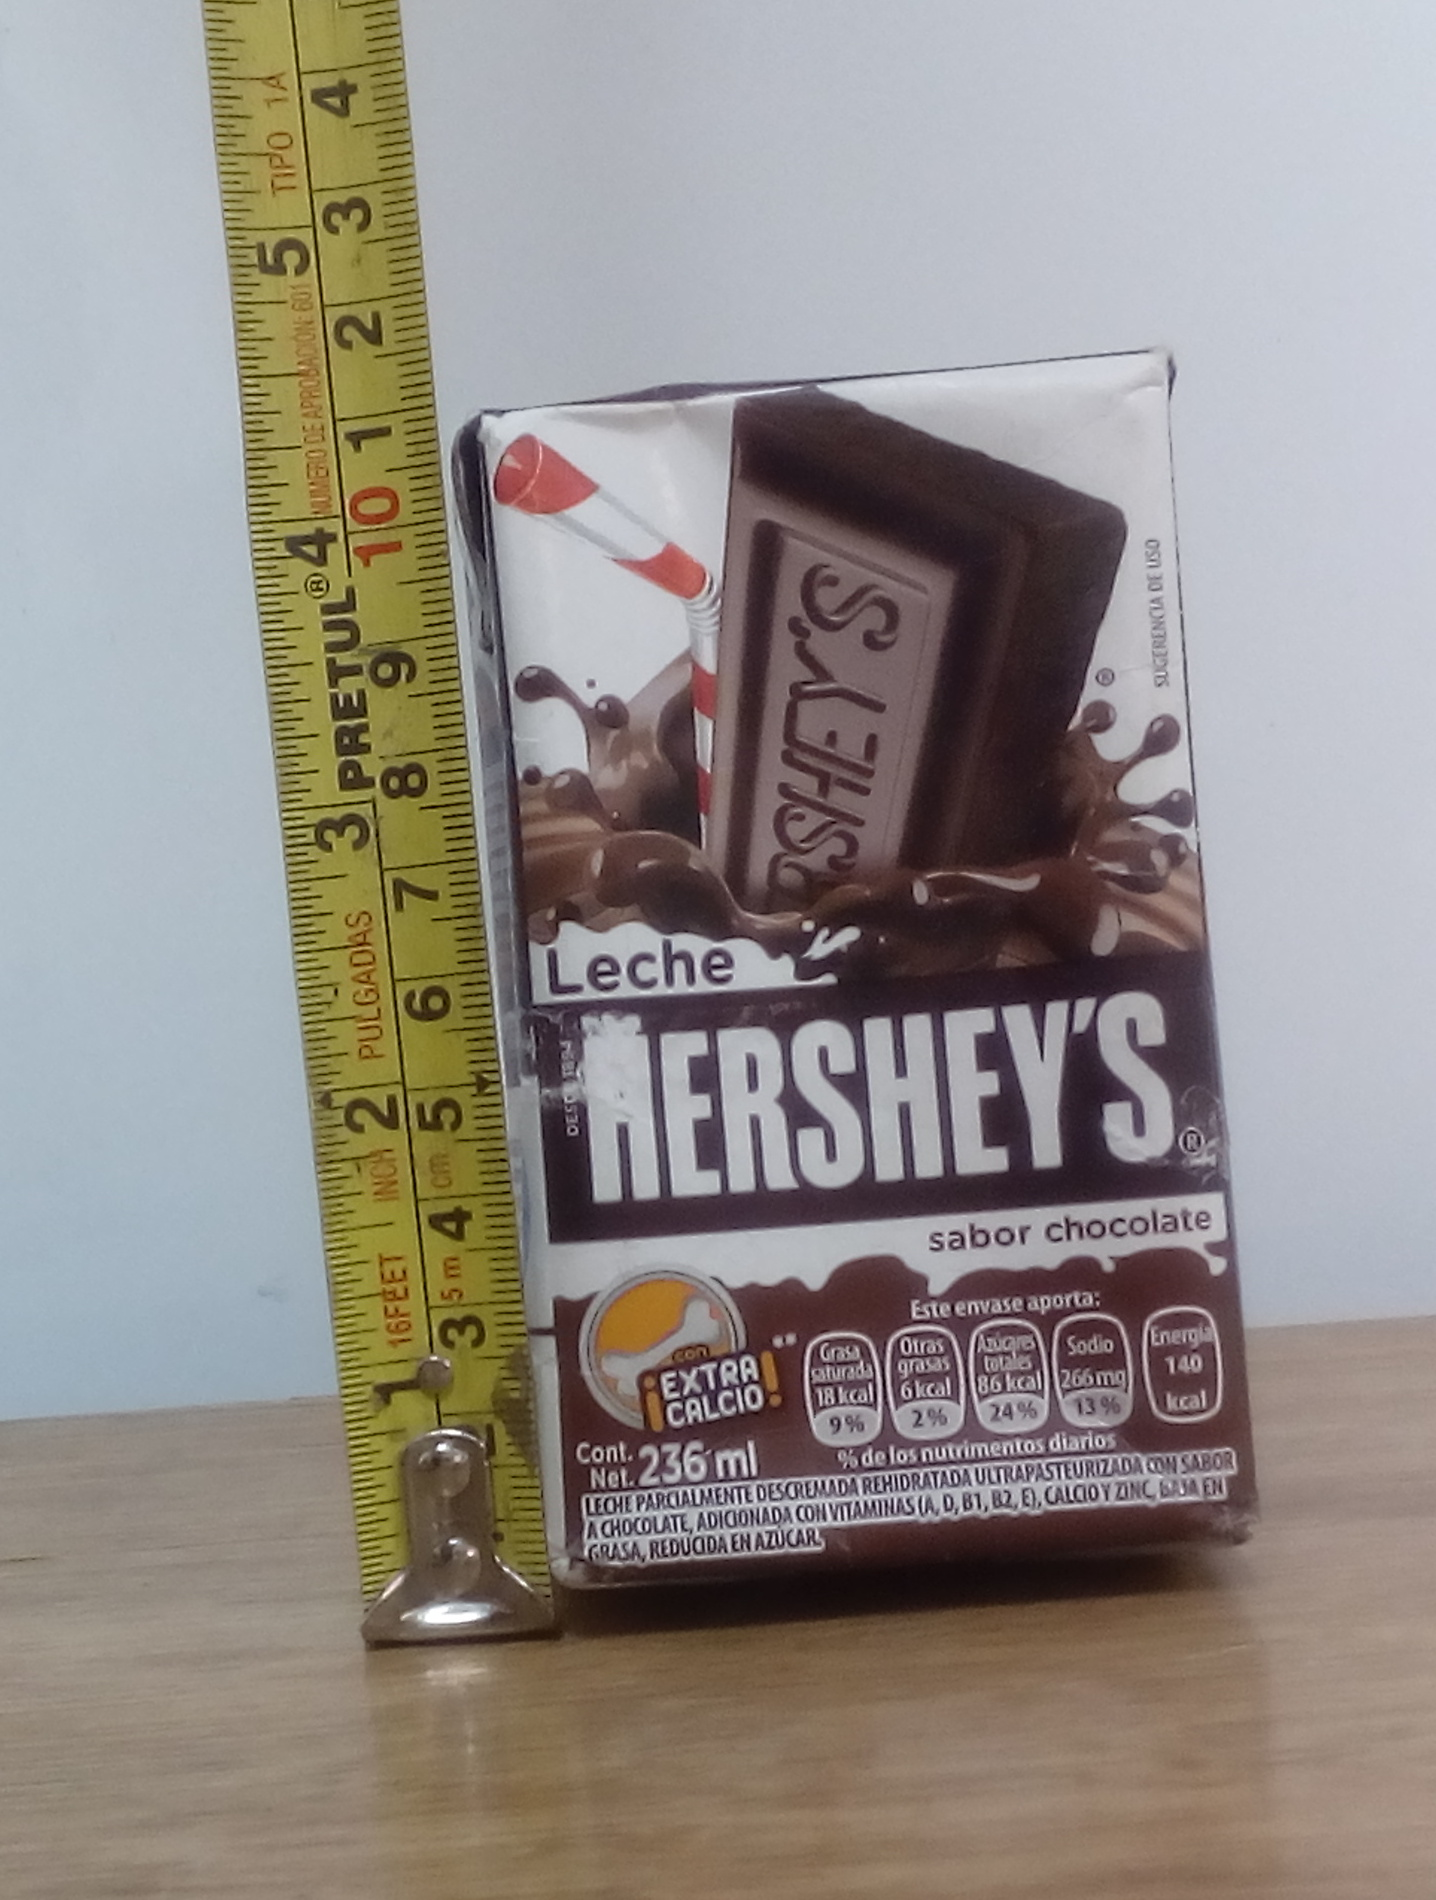
\includegraphics[scale=0.06]{objs_real/milkHeight.jpg}	
		\end{subfigure}%
		\begin{subfigure}[h]{.5\textwidth}
		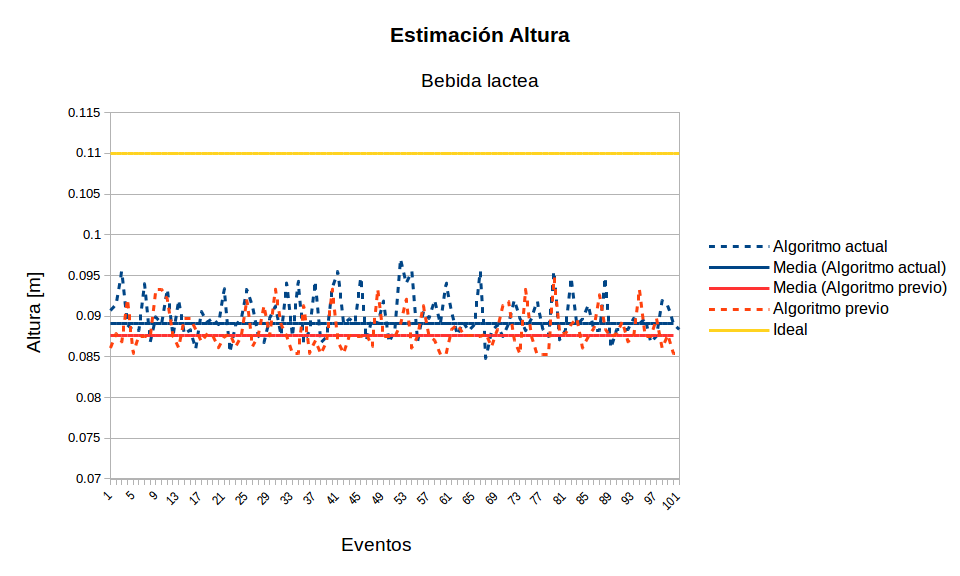
\includegraphics[scale=0.45]{resultados/lecheAltura_media.png}	
		\end{subfigure}
		\caption{Gráficas de estímaciones de alturas para un envase de leche. La altura real del objeto (amarillo), la altura estímada con el algoritmo previo (rojo) y la estimación actual (azul).}
		\label{fig:mesh1}
	\end{figure}

	\begin{figure}[H]
		\begin{subfigure}[h]{.30\textwidth}
		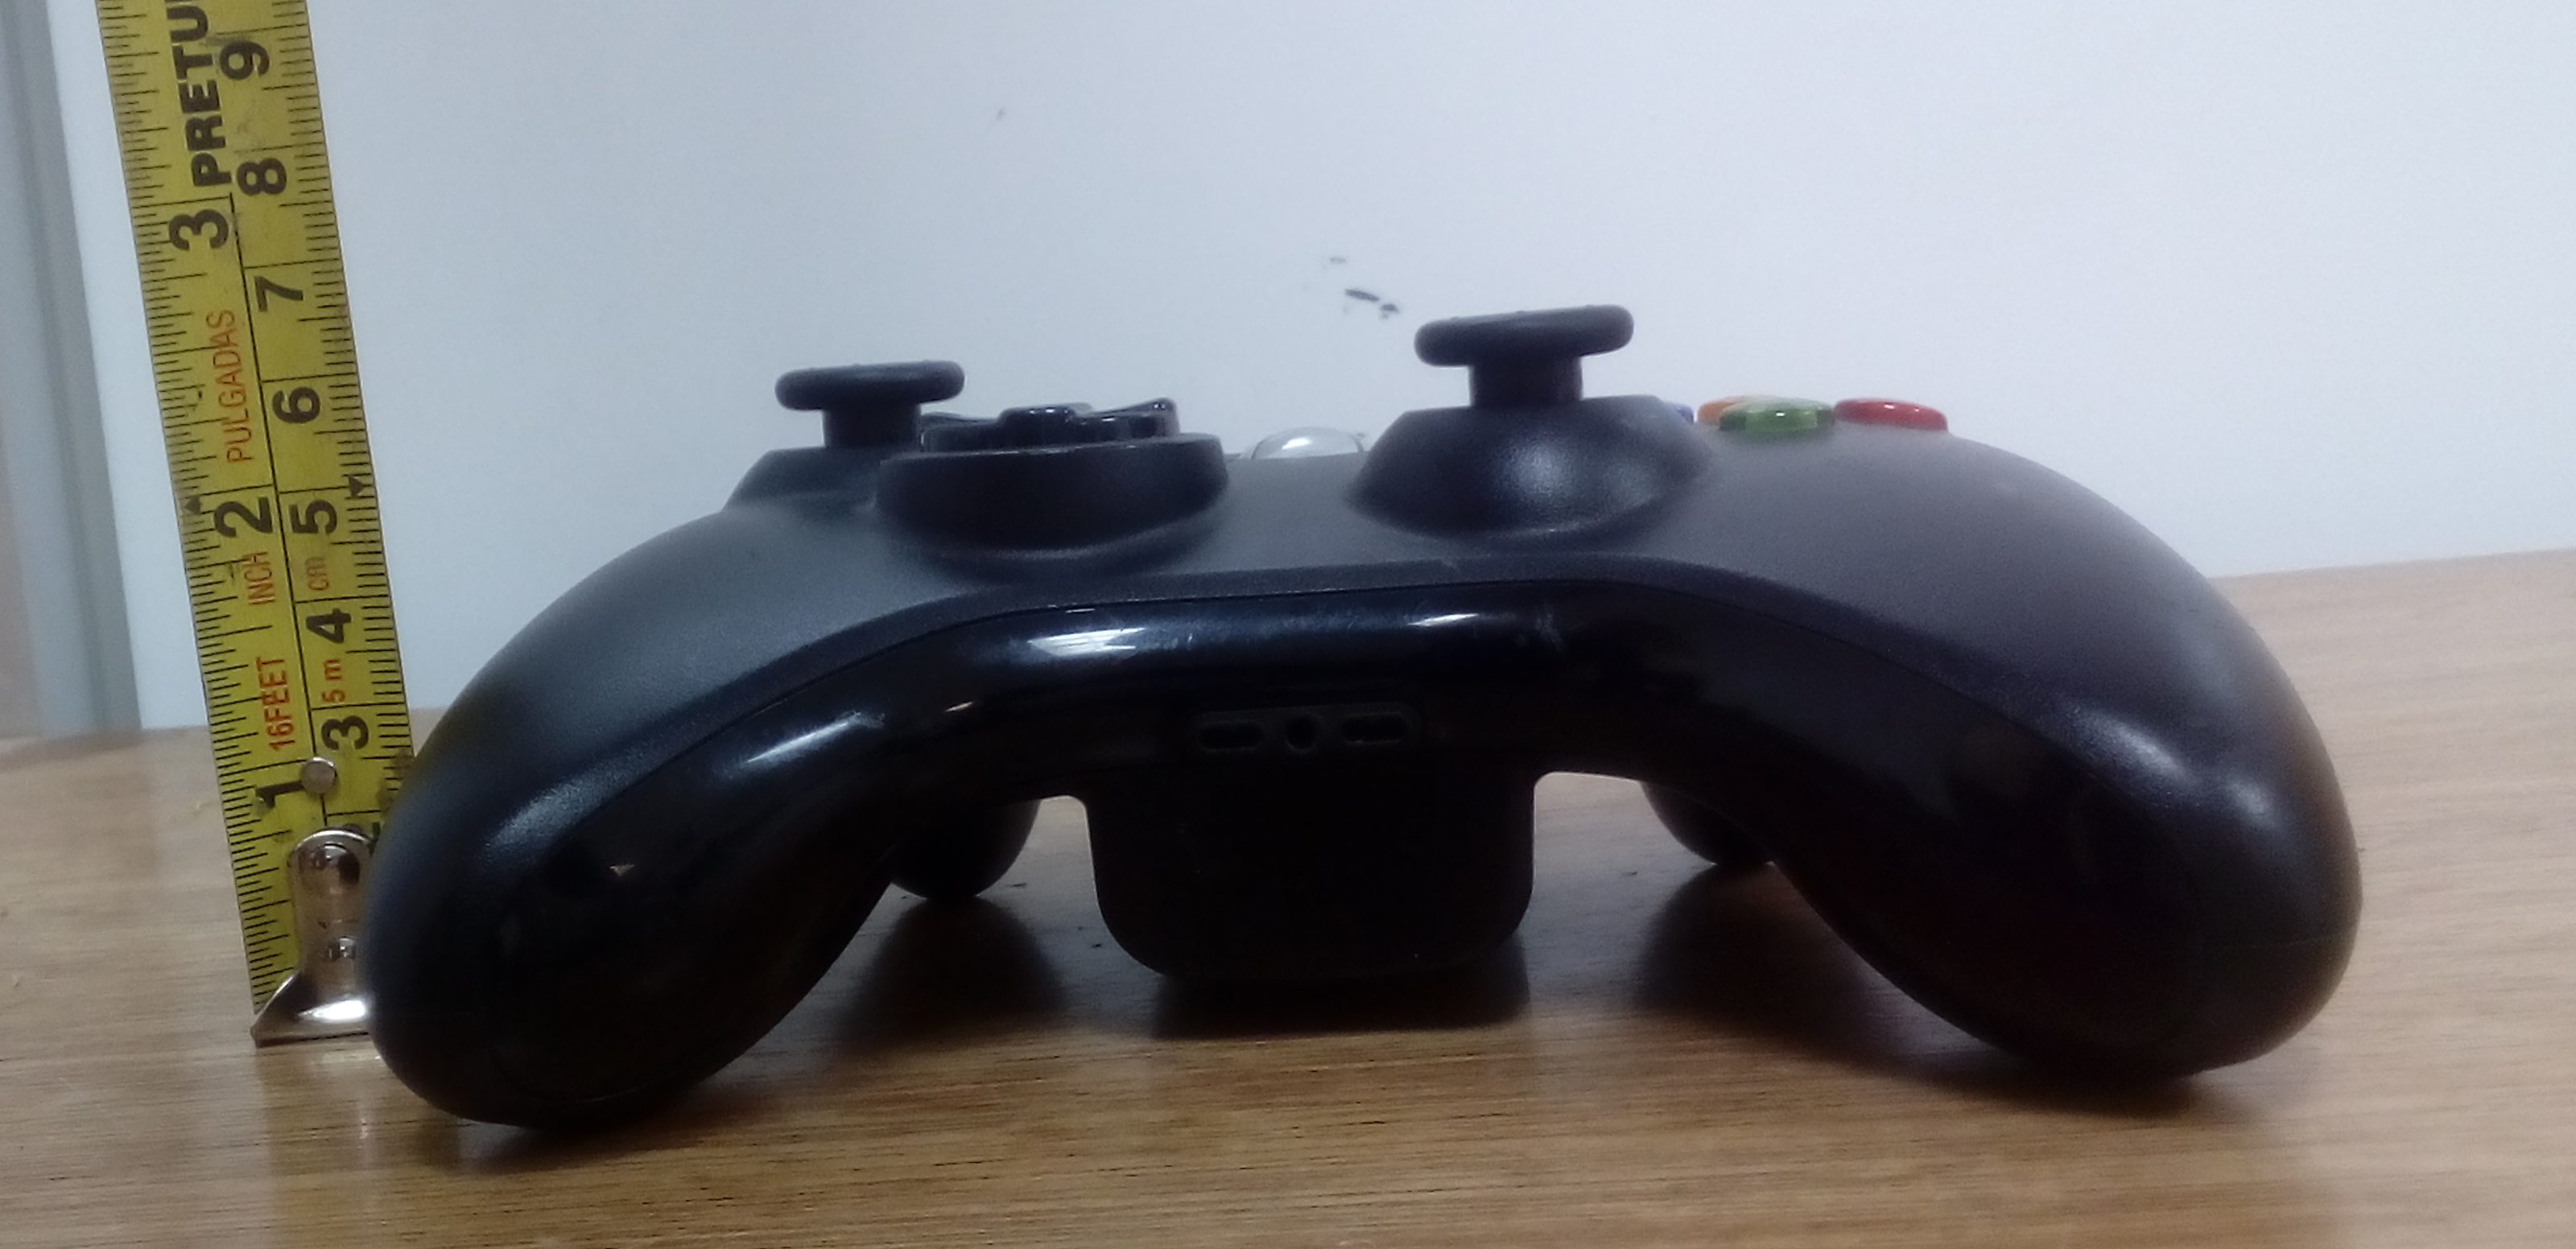
\includegraphics[scale=0.04]{objs_real/joystickHeight2.jpg}	
		\end{subfigure}%
		\begin{subfigure}[h]{.5\textwidth}
		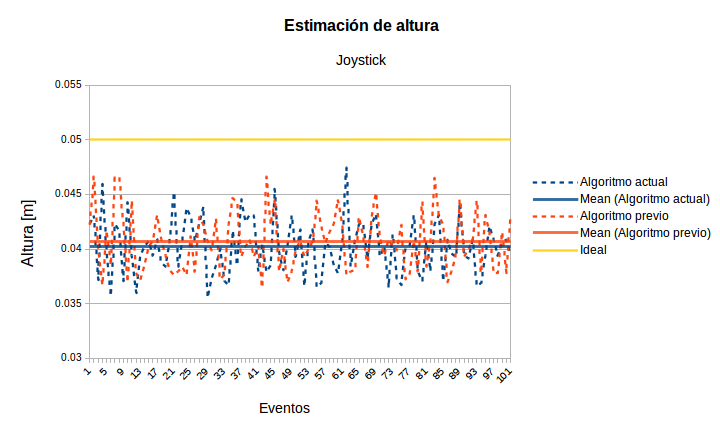
\includegraphics[scale=0.45]{resultados/joystickAltura_media.png}	
		\end{subfigure}
		\caption{Gráficas de estímaciones de alturas para un control de videojuegos. La altura real del objeto (amarillo), la altura estímada con el algoritmo previo (rojo) y la estimación actual (azul).}
		\label{fig:mesh1}
	\end{figure}

	\begin{figure}[H]
		\begin{subfigure}[h]{.30\textwidth}
		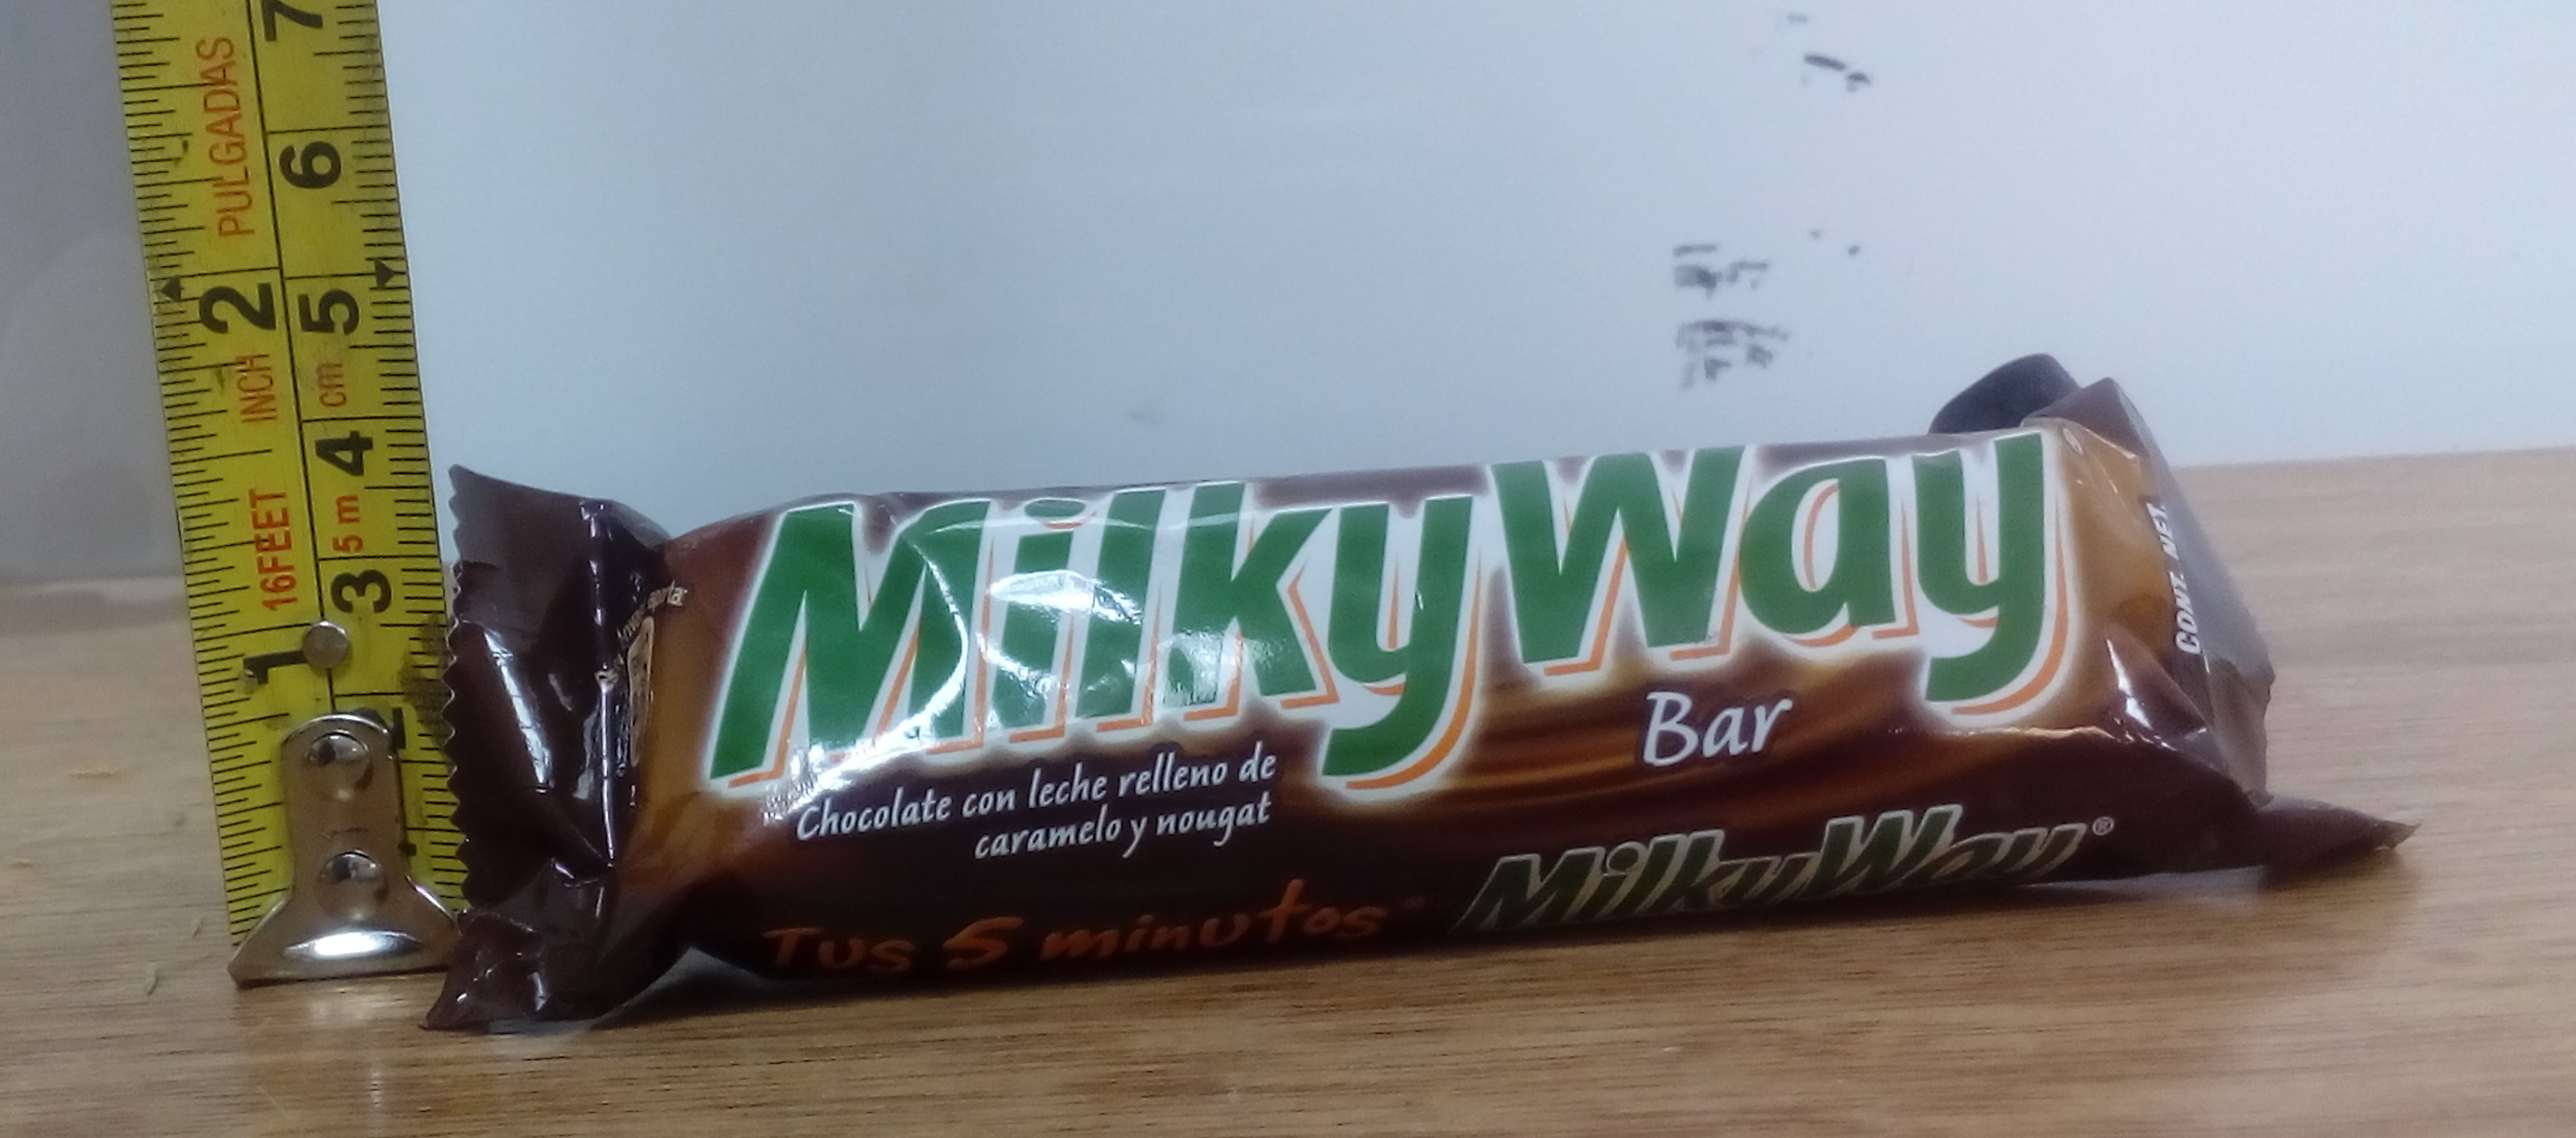
\includegraphics[scale=0.04]{objs_real/chocolateHeight2.jpg}	
		\end{subfigure}%
		\begin{subfigure}[h]{.5\textwidth}
		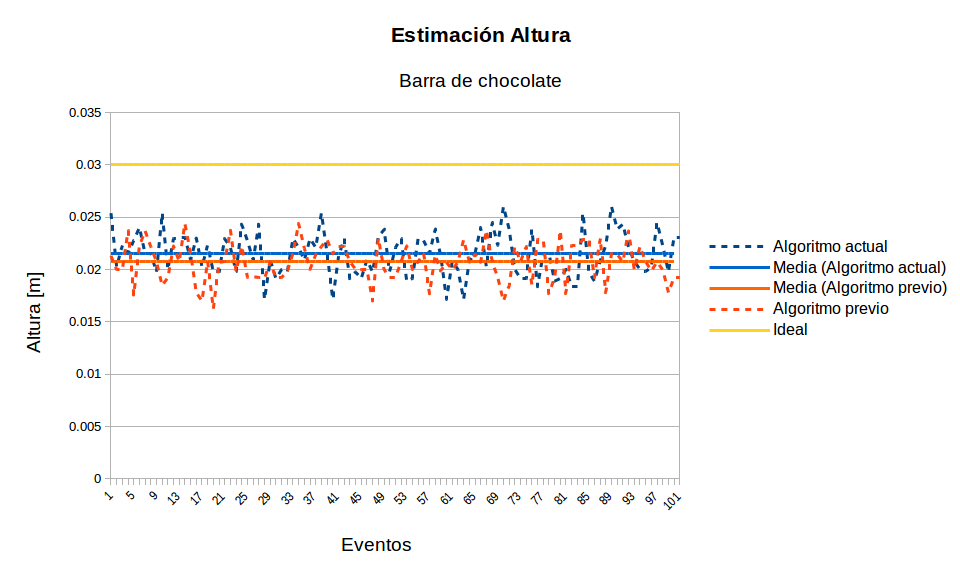
\includegraphics[scale=0.45]{resultados/chocolateAltura_media.png}	
		\end{subfigure}
		\caption{Gráficas de estímaciones de alturas para una barra de chocolate. La altura real del objeto (amarillo), la altura estímada con el algoritmo previo (rojo) y la estimación actual (azul).}
		\label{fig:mesh1}
	\end{figure}

	Posteriormente, se realizó una prueba T para muestras pareadas (prueba t de mediciones repetidas) con la cual podemos obtener información sobre las diferencias de medias, pero sobre todo podemos saber si son significativamente difereentes. En el caso de este trabajo es necesario saber si las medias de las muestras tomadas realmente representan una mejor estimación de alturas.\\

	A continuación se reportan los valores de medias, con el valor T obtenido para cada conjunto de pruebas (altura estimada por algoritmo previo contra altura estimada por algoritmo actual).

\begin{table}[H]
	\centering
	\begin{tabular}{ |p{2.0cm}|p{2.0cm}|p{2.0cm}|p{2.0cm}|p{2.0cm}|p{2.0cm}|  }
	 \hline
	 & \multicolumn{2}{|c|}{\textbf{Algoritmo previo} } & \multicolumn{2}{|c|}{\textbf{Algoritmo actual}} &\\
	 \hline
	 \textbf{Objeto} &\textbf{Altura media [m]}  &\textbf{Varianza}&\textbf{Altura media [m]}  &\textbf{Varianza} & \textbf{$P_{value}$}\\
	 \hline
	  Cereal    &	 0.2568  & $1.79e^{-6}$ & 0.2324 & $4.22e^{-6}$ & $p_{value} < 2.2e^{-16}$  \\
	 \hline
	  Jugo      &    0.1407  & $3.28e^{-6}$ & 0.1305 & $1.67e^{-6}$ & $p_{value} < 2.1e^{-16}$  \\
	 \hline
	  Leche     &    0.0901  & $7.33e^{-6}$ & 0.0889 & $5.54e^{-6}$ &$p_{value} < 2.1e^{-16}$  \\
	 \hline 
	  Control de videojuegos &  0.0485  & $6.28e^{-6}$ &0.0411 & $7.01e^{-6}$ & $p_{value} = 0.0175$ \\
	 \hline
	  Barra de chocolate   &    0.0215  & $3.3e^{-6}$  &0.0213 & $4.4e^{-6}$ & $p_{value} = 0.1335$ \\
	 \hline
	\end{tabular}
	\caption{Tabla de resultados de la prueba T a medidas repetidas.}
	\label{t_test:1}
\end{table}




\newpage
%%%%%%%%%%%%%%%%%%%%%%%%%%%%%%%%%%%%%%%%%%%%%%%%%%%%%%%%%%%%
%%%%%%%%% Cálculo de las orientaciones  %%%%%%%%%%%%%%%%%%%%
	\section{Cálculo de la orientación del objeto.}

	En esta sección del trabajo se reportan los resultados obtenidos al realizar las preubas de estimación de orientación de los objetos sobre un plano, para ser más exactos objetos sobre una mesa. En esta prueba se realizaron 50 tomas de datos para cada uno de los obetos con direferentes orientaciones.\\

	El proceso para poner a prueba la estimación de ángulos de los objetos con respecto del eje Y del robot se describe a continuación. Una vez obtenidos los vectores propios de la matriz de covarianzas, se obtien un conjunto de vectores ortogonales que nos indican los ejes en los cuales sucede la mayor distribución de puntos de un objeto. Con este conjunto de vectores se realizaron dos procesos:\\

	\begin{itemize}
		\item{Un ordemaniento por magnitud.}
		\item{Una ordenamiento por magnitudes en las respectivas componentes $x, y, z$}
	\end{itemize}  

		Con la información de los vectores ordenados se puede comparar si el mayor eje de distribución ocurre en el eje $z$ del robot o si ocurre en alguno de los vectores paralelos al conjunto de vectores que definirían el plano sobre el cual se encuentran los objetos.\\

		El algoritmo para calcular el ángulo del objeto con respecto del eje $y$ del robot, se explica de la siguiente manera: se toma el vector paralelo al plano con mayor magnitud, puesto que sabemos del ordenamiento cual es el vector en el mayo eje z descartamos este del proceso, con los dos vectores restantes obtenemos el de mayor magnitud.\\

		Este vector apuntaría en la direccción $y$ o $-y$ para un caso ideal en que el ángulo del objeto fuera de cero grados con respecto del eje $y$ del robot. en este punto se realiza un acotamiento para que dicho vector apunte hacia el eje $y$ del robot, posteriormente se calcula el ángulo de rotación por medio del producto punto que existe entre el ángulo del vector estimado para el objeto y el vector que apunta en la dirección del vector unitario $y$ del robot.\\


		%\newpage
		\subsection{Pruebas para objetos a 0 grados}

		Los resultados que se obtuvieron de la prueba antes mencionada, se muestran en las gráficas posteriores en este documento. 

		\begin{figure}[H]
			\centering
			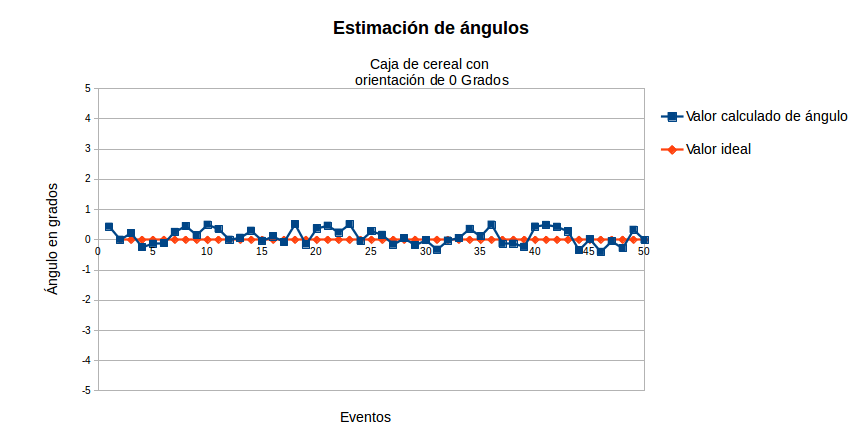
\includegraphics[scale=0.40]{resultados/angulos_cereal.png}
			\caption{Gráficas de estímaciones de ángulos para una caja de cereal con orientación de 0 grados respecto al eje $y$ del robot.}
			\label{fig:mesh1}
		\end{figure}

		\begin{figure}[H]
			\centering
			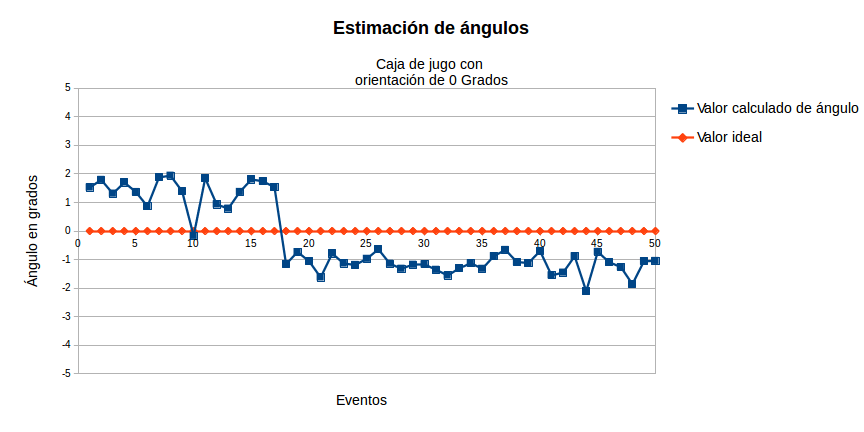
\includegraphics[scale=0.40]{resultados/angulos_jugo.png}
			\caption{Gráficas de estímaciones de ángulos para una caja de jugo con orientación de 0 grados respecto al eje $y$ del robot.}
			\label{fig:mesh1}
		\end{figure}

		\begin{figure}[H]
			\centering
			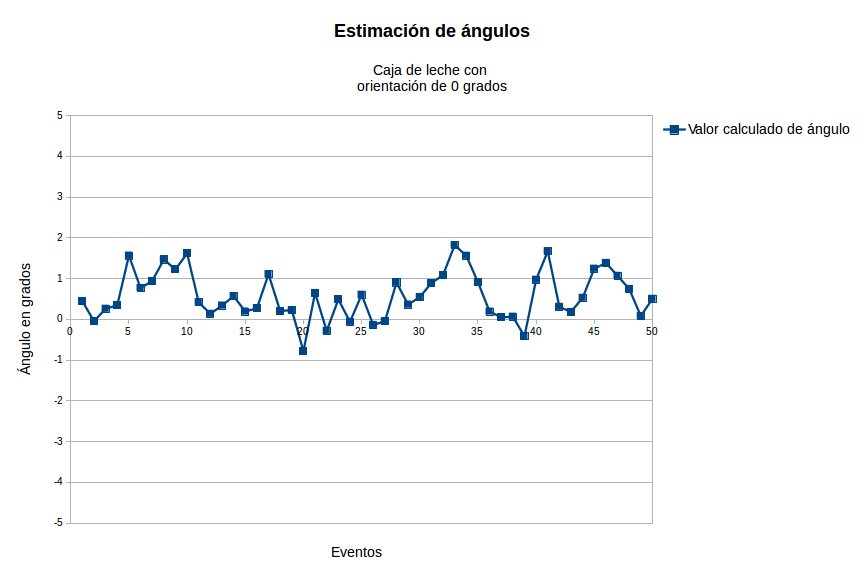
\includegraphics[scale=0.40]{resultados/angulos_milk.png}
			\caption{Gráficas de estímaciones de ángulos para una caja de leche con orientación de 0 grados respecto al eje $y$ del robot.}
			\label{fig:mesh1}
		\end{figure}

		\begin{figure}[H]
			\centering
			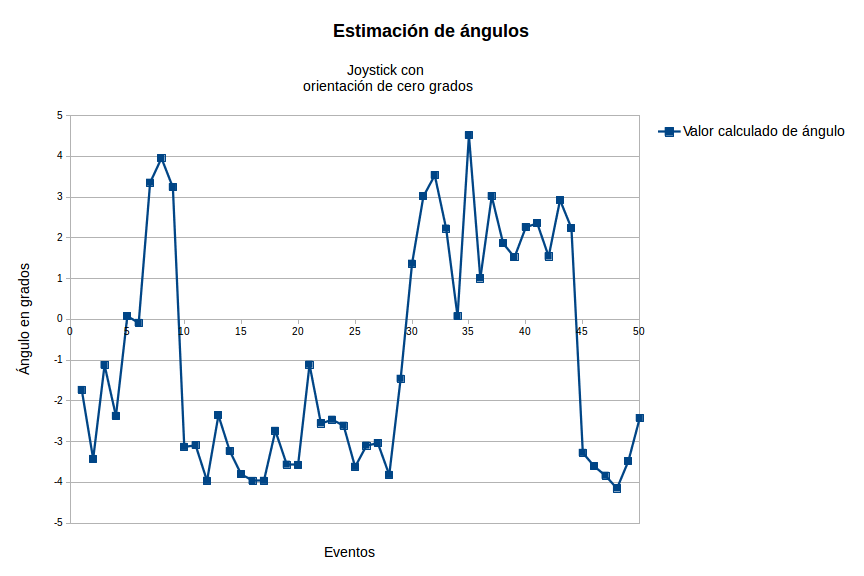
\includegraphics[scale=0.40]{resultados/angulos_joystick.png}
			\caption{Gráficas de estímaciones de ángulos para un control de videojuegos con orientación de 0 grados respecto al eje $y$ del robot.}
			\label{fig:mesh1}
		\end{figure}

		\begin{figure}[H]
			\centering
			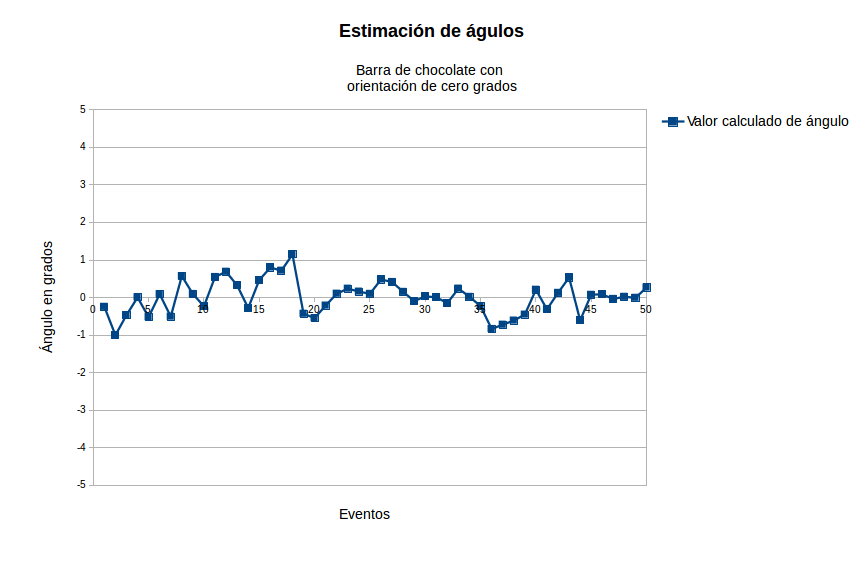
\includegraphics[scale=0.40]{resultados/angulos_chocolate.png}
			\caption{Gráficas de estímaciones de ángulos para una barra de chocolate con orientación de 0 grados respecto al eje $y$ del robot.}
			\label{fig:mesh1}
		\end{figure}



		\newpage
		%%%%%%%%%%%%%%%%%%%%%%%%%%%%%%%%%%%%%%%%%%%%%%%%%%%%%%%%%%%%%%%%%
		% PRUEBAS A 45 GRADOS %
		\subsection{Pruebas para objetos a 45 grados}

		\begin{figure}[H]
			\centering
			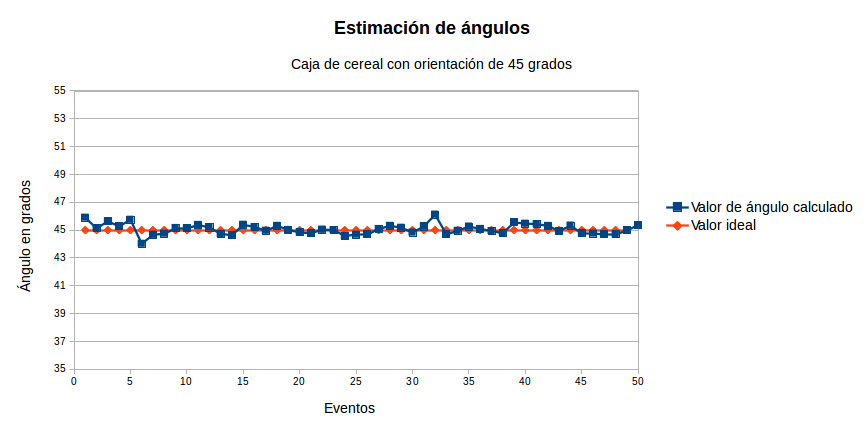
\includegraphics[scale=0.40]{resultados/angulos_cereal_45.png}
			\caption{Gráficas de estímaciones de ángulos para una caja de cereal con orientación de 45 grados respecto al eje $y$ del robot.}
			\label{fig:mesh1}
		\end{figure}

		\begin{figure}[H]
			\centering
			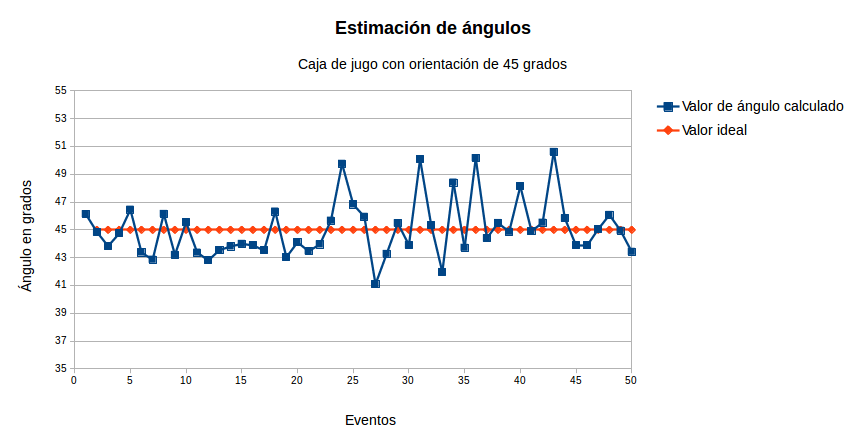
\includegraphics[scale=0.40]{resultados/angulos_jugo_45.png}
			\caption{Gráficas de estímaciones de ángulos para una caja de jugo con orientación de 45 grados respecto al eje $y$ del robot.}
			\label{fig:mesh1}
		\end{figure}

		\begin{figure}[H]
			\centering
			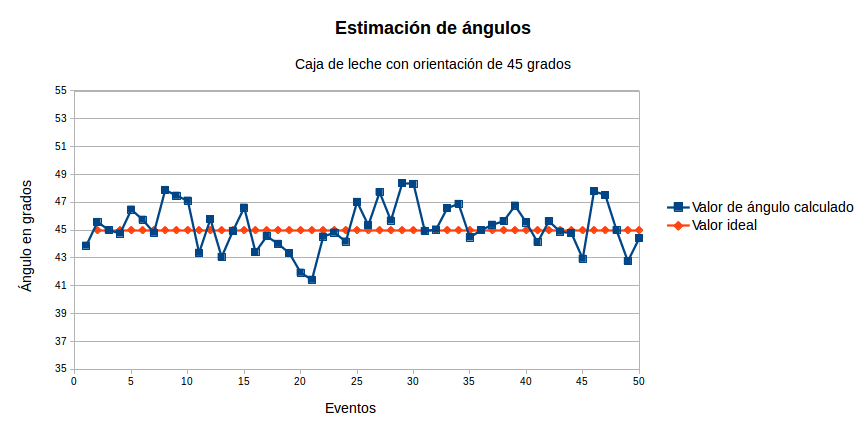
\includegraphics[scale=0.40]{resultados/angulos_milk_45.png}
			\caption{Gráficas de estímaciones de ángulos para una caja de leche con orientación de 45 grados respecto al eje $y$ del robot.}
			\label{fig:mesh1}
		\end{figure}

		\begin{figure}[H]
			\centering
			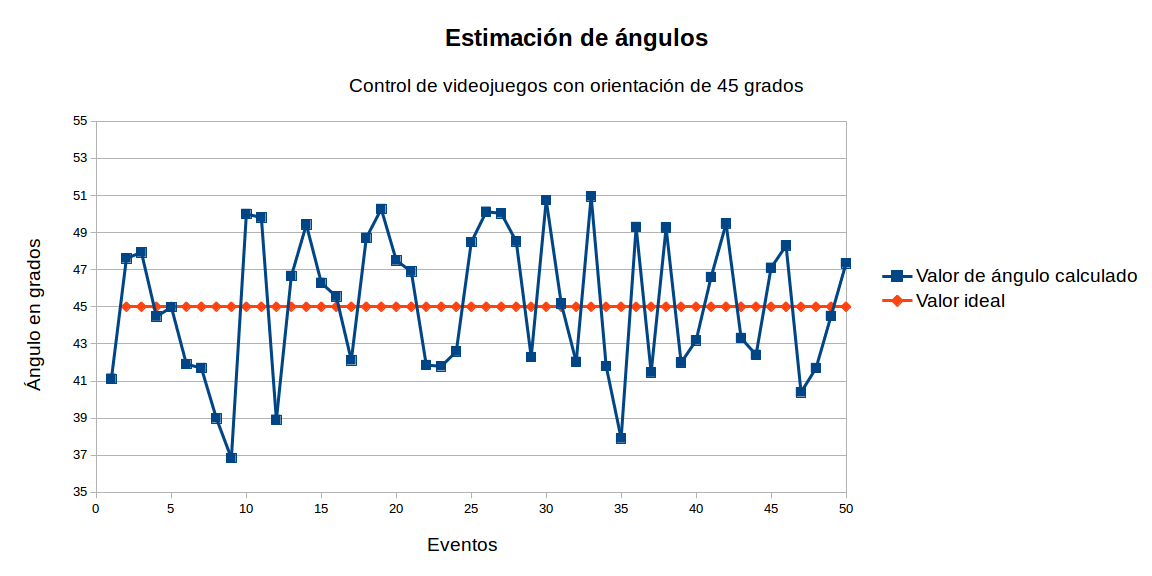
\includegraphics[scale=0.40]{resultados/angulos_joystick_45.png}
			\caption{Gráficas de estímaciones de ángulos para un control de videojuegos con orientación de 45 grados respecto al eje $y$ del robot.}
			\label{fig:mesh1}
		\end{figure}

		\begin{figure}[H]
			\centering
			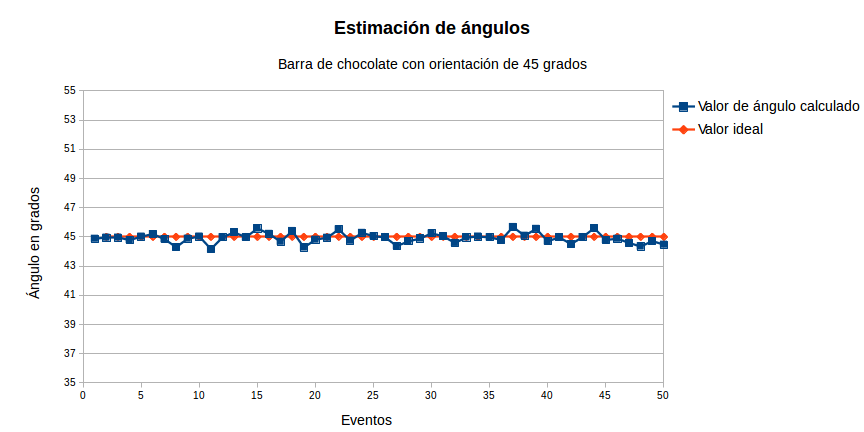
\includegraphics[scale=0.40]{resultados/angulos_chocolate_45.png}
			\caption{Gráficas de estímaciones de ángulos para una barra de chocolate con orientación de 45 grados respecto al eje $y$ del robot.}
			\label{fig:mesh1}
		\end{figure}



		\newpage
		%%%%%%%%%%%%%%%%%%%%%%%%%%%%%%%%%%%%%%%%%%%%%%%%%%%%%%%%%%%%%%%%%
		%%%%%%%%%%%%%%         PRUEBAS A 90 GRADOS       %%%%%%%%%%%%%%%
		\subsection{Pruebas para objetos a 90 grados}
		\begin{figure}[H]
			\centering
			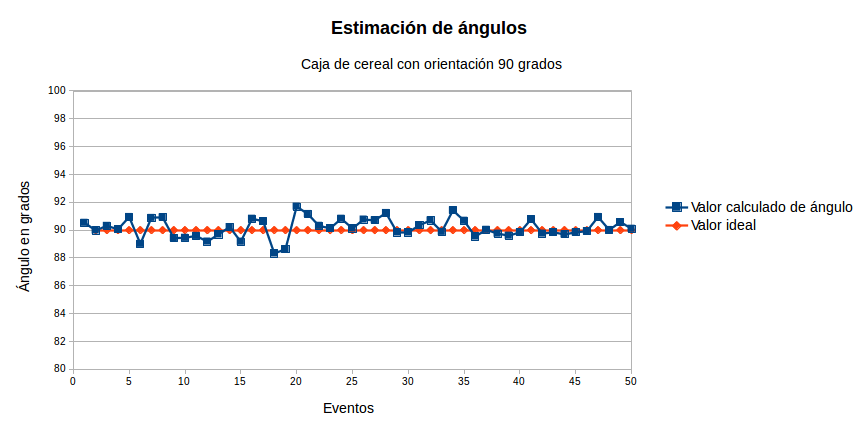
\includegraphics[scale=0.40]{resultados/angulos_cereal_90.png}
			\caption{Gráficas de estímaciones de ángulos para una caja de cereal con orientación de 90 grados respecto al eje $y$ del robot.}
			\label{fig:mesh1}
		\end{figure}

		\begin{figure}[H]
			\centering
			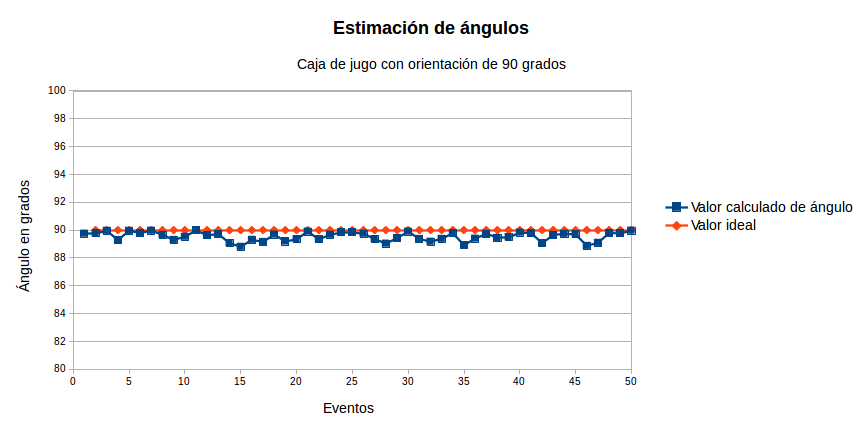
\includegraphics[scale=0.40]{resultados/angulos_jugo_90.png}
			\caption{Gráficas de estímaciones de ángulos para una caja de jugo con orientación de 90 grados respecto al eje $y$ del robot.}
			\label{fig:mesh1}
		\end{figure}

		\begin{figure}[H]
			\centering
			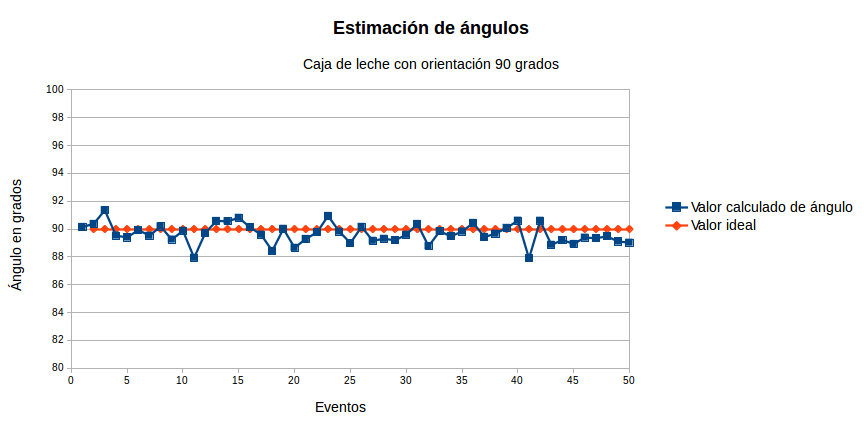
\includegraphics[scale=0.40]{resultados/angulos_milk_90.png}
			\caption{Gráficas de estímaciones de ángulos para una caja de leche con orientación de 90 grados respecto al eje $y$ del robot.}
			\label{fig:mesh1}
		\end{figure}

		\begin{figure}[H]
			\centering
			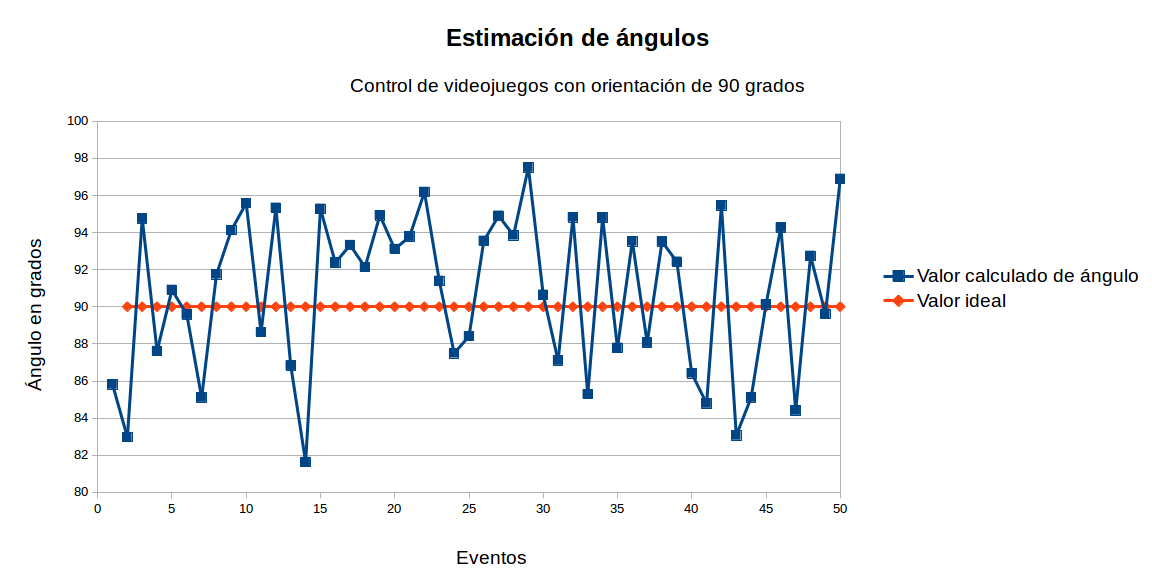
\includegraphics[scale=0.40]{resultados/angulos_joystick_90.png}
			\caption{Gráficas de estímaciones de ángulos para un control de videojuegos con orientación de 90 grados respecto al eje $y$ del robot.}
			\label{fig:mesh1}
		\end{figure}

		\begin{figure}[H]
			\centering
			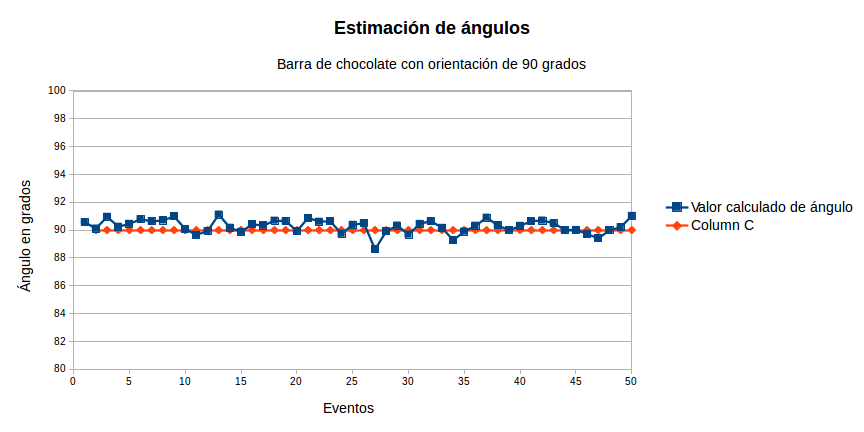
\includegraphics[scale=0.40]{resultados/angulos_chocolate_90.png}
			\caption{Gráficas de estímaciones de ángulos para una barra de chocolate con orientación de 90 grados respecto al eje $y$ del robot.}
			\label{fig:mesh1}
		\end{figure}

	A continuación se muestran las tablas con los datos de las varianzas de los datos y los errores medios cuadráticos de los datos obtenidos con respecto de los valores esperados.\\




\newpage
%%%%%%%%%%%%%%%%%%%%%%%%%%%%%%%%%%%%%%%%%%%%%%%%%%%%%%%%%%%
%%%%%%%%%% PRUEBAS DE GRASPEO CON INFORMACIÓN DEL ÁREA DE TRABAJO  %%%%%%%%%%%%
	\section{Tiempo de ejecución para diferentes algoritmos de cinemática inversa.}
	Como parte de este trabajo se propone evaluar y comparar el desempeño de dos algoritmos empleados para el cálculo de la cinemática inversa de un manipulador de 7 grados de libertad. Para ello se puso a prueba un método geométrico desarrollado previamente, con motivo de este trabajo se implementó una instacia de solución con la paquetería moveIt!. La paquetería moveIt! ofrece una solución numerica de cinemáticas para manipualdores. En este caso se puso a prueba el solucionador OMPL.\\

	El trabajo de esta tesis, en este apartado, fue crear un modelo matemático del manipulador de 7 grados de libertad, para posteriormente poner a prueba su rapidez de solución y su robuztes para calcular la cinemática inversa.\\ 

	A continuación se reportan los resultados obtenidos. Se muestran gráficas de rapidez de ejecución, cantidad de puntos para los cuales ambos métodos encontraron solución y el valor de una función de costo represantiva de una función de energía requeida para mover el manipulador.\\ 

	\subsection{Tiempo de ejecución para diferentes algoritmos de cinemática inversa.}

	En esta sección se reportan los resultados obtenidos de evaluar la función de costo para los respectivos algoritmos del cálculo de la cinemática inversa. En la figura \ref{fig:successIK} se muestran los resultados del tiempo de ejecución para en el caso en que ambos algoritmos encontraron una solución. Notamos que no difieren más de 1 [ms], por tanto es un tiempo de ejecución aceptable.\\

	Por otro lado, en la figura \ref{fig:unsuccessIK} se reportan los tiempos de ejecución en el caso que los algoritmos no encotraron una solución. Podemos observar en el caso del algoritmo iterativo que supera un tiempo de 3[s] aproximadamente. Lo cual es totalmente inconveniente si lo que se requiere es velocidad de respuesta.\\

	\begin{figure}[H]
		\centering
		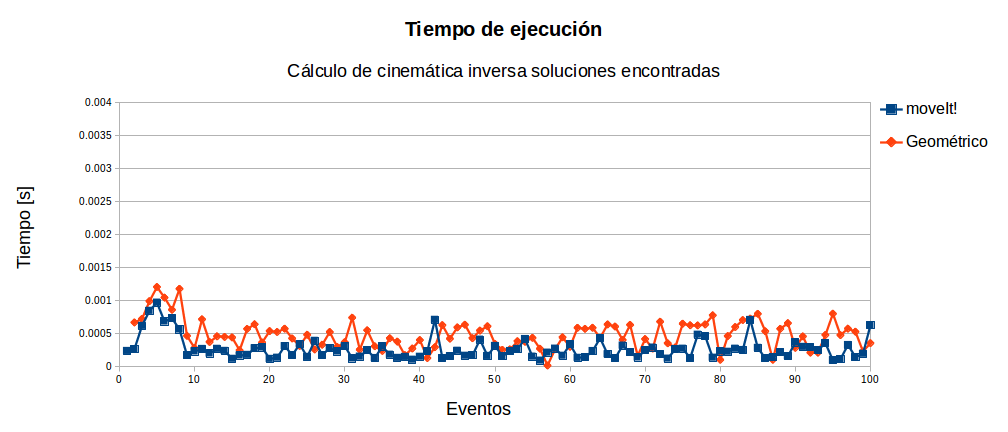
\includegraphics[scale=0.50]{resultados/success_IKcalculate.png}
		\caption{Gráfica de tiempo de ejecución para el cálculo de la cinemática inversa por metodo geométrico(rojo) y por método númerico (azul). Caso de solución encontrada.}
		\label{fig:successIK}
	\end{figure}

	\begin{figure}[H]
		\centering
		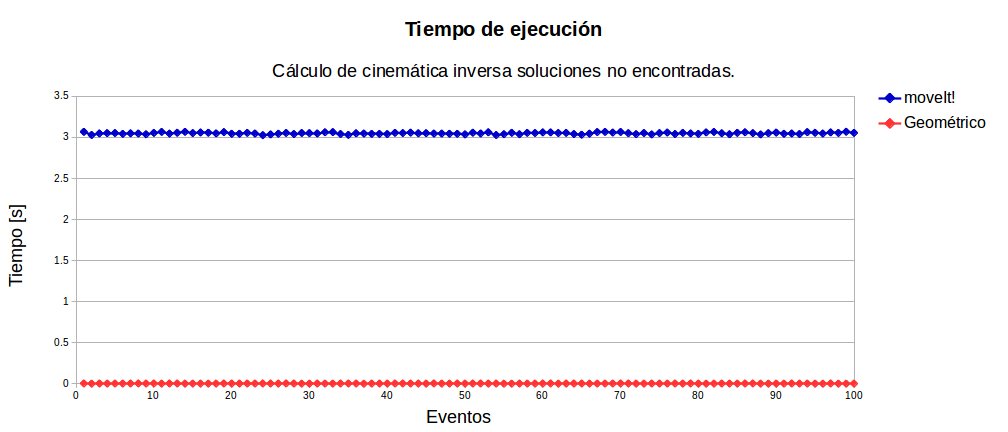
\includegraphics[scale=0.50]{resultados/unsuccess_IKcalculate.png}
		\caption{Gráfica de tiempo de ejecución para el cálculo de la cinemática inversa por metodo geométrico(rojo) y por método númerico (azul). Caso de \textbf{solución no encontrada.} } 
		\label{fig:unsuccessIK}
	\end{figure}

	

	\subsection{Prueba de robustez y evalución del valor de la funcion de costo.}

	Otra de las pruebas que se realizaron con la finalidad de comparar los algoritmos de cálculo de cinemática inversa fue la evaluación de una función de costo. Esta fucnión esta planteada en terminos de un mínimo consumo energético. En la figura \ref{fig:funcCost} se muestra el valor resultante de evaluar la función (4.14) para diferentes puntos cartesianos.\\ 

	En gráfica \ref{fig:histFuncCost} se muestra la cantidad de ocasiones en que fue menor el valor de dica función para cada uno de los algoritmos. De lo cual observamos que el método geométrico obtivo un menor valor en 59 ocasiones, por otro lado el algoritmo iterativo solo obtuvo un menor valor en 4 ocasiones. Estas pruebas se realizaron un total de 150 ocasiones, en las cuales el algoritmo iterativo solo encontró solución 63 ocasiones, como se muestra en la figura \ref{fig:iIKsuccess}.\\

	\begin{figure}[H]
		\centering
		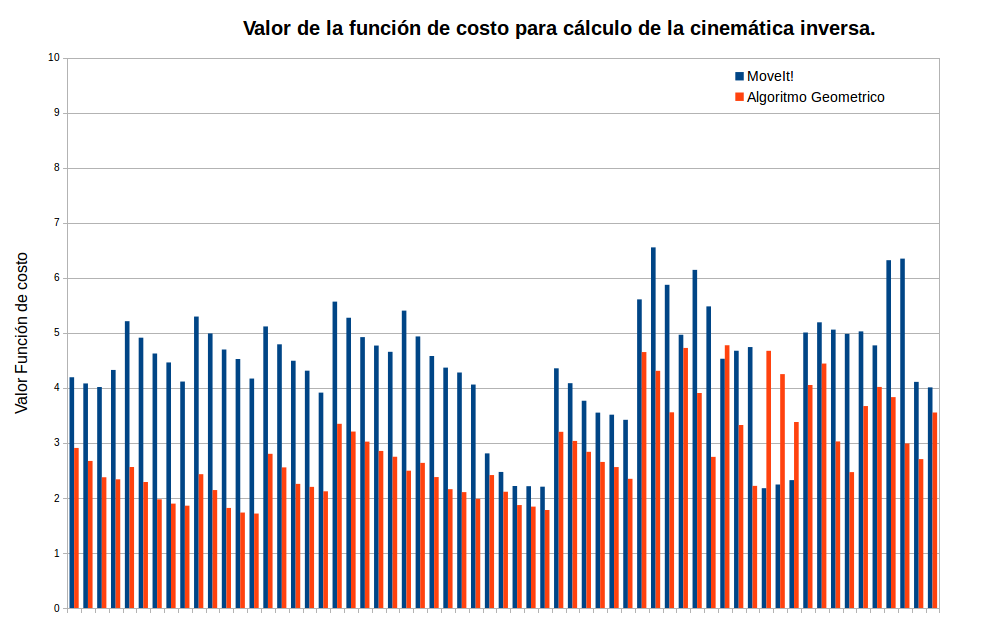
\includegraphics[scale=0.45]{resultados/valor_costFunction.png}
		\caption{Gráficas comparativa de la función de costo para diferentes algoritmos de la cinemática inversa.}
		\label{fig:funcCost}
	\end{figure}

	\begin{figure}[H]
		\centering
		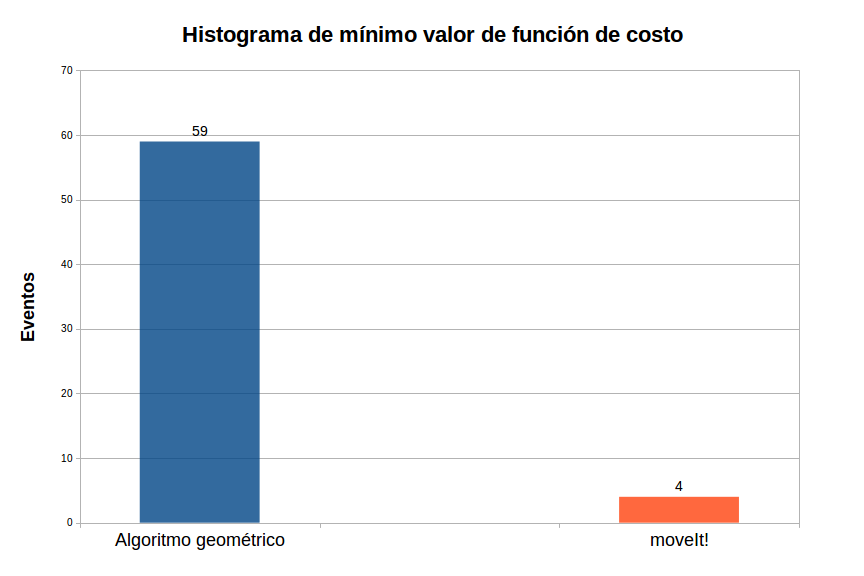
\includegraphics[scale=0.45]{resultados/hist_valor_costFunction.png}
		\caption{.}
		\label{fig:histFuncCost}
	\end{figure}

	\begin{figure}[H]
		\centering
		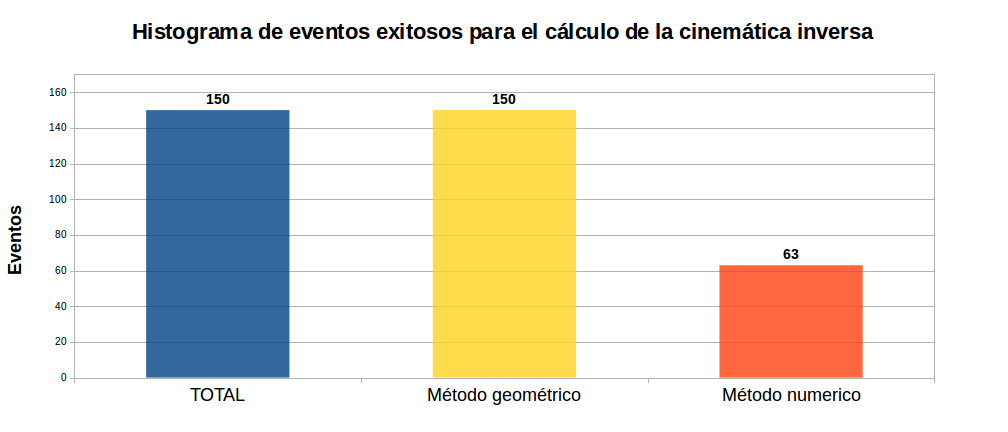
\includegraphics[scale=0.45]{resultados/histograma_success.png}
		\caption{Gráficas de estímaciones de ángulos para una barra de chocolate con orientación de 90 grados respecto al eje $y$ del robot.}
		\label{fig:iIKsuccess}
	\end{figure}



\newpage
%%%%%%%%%%%%%%%%%%%%%%%%%%%%%%%%%%%%%%%%%%%%%%%%%%%%%%%%%%%%%%%%%%%%%%%%%%%%%%
%%%%%%%%%% PRUEBAS GRASPEO CON DIFERENTES INFORMACIONES %%%%%%%%%%%%
	\section{Pruebas de manipulación con el robot real}

	Como reporte último de las pruebas, se realizaron pruebas físicas con el robot de servicio Justina. Para tener una prueba estadistica que pueda servir de compración se realizaron un total de 70 eventos, divididos en 10 repeticiones para 6 objetos. Los objetos con los cuales se realizaon las pruebas fueron: una caja de cereal, un envase de jugo, un envase de bebida lactea, un control de videojuegos, una barra de chocolate, un libro y una bolsa de cartón.\\

	Las orientaciones de los objetos en cada uno de los eventos fueron posiciones aleatorias. Esto con el fin de poner a prueba las características de presición en la orientación de los objetos para este algoritmo.\\
	

	En la primer parte de la prueba se realizó la toma de objetos sin considerar la información de la orientación. Y en la segunda fase se realizaon las respectivas pruebas considerando la información de la orientación.\\

	\begin{figure}[H]
		\hspace*{-0.3in}
		\centering
		\begin{subfigure}[t]{.55\textwidth}
			\centering
			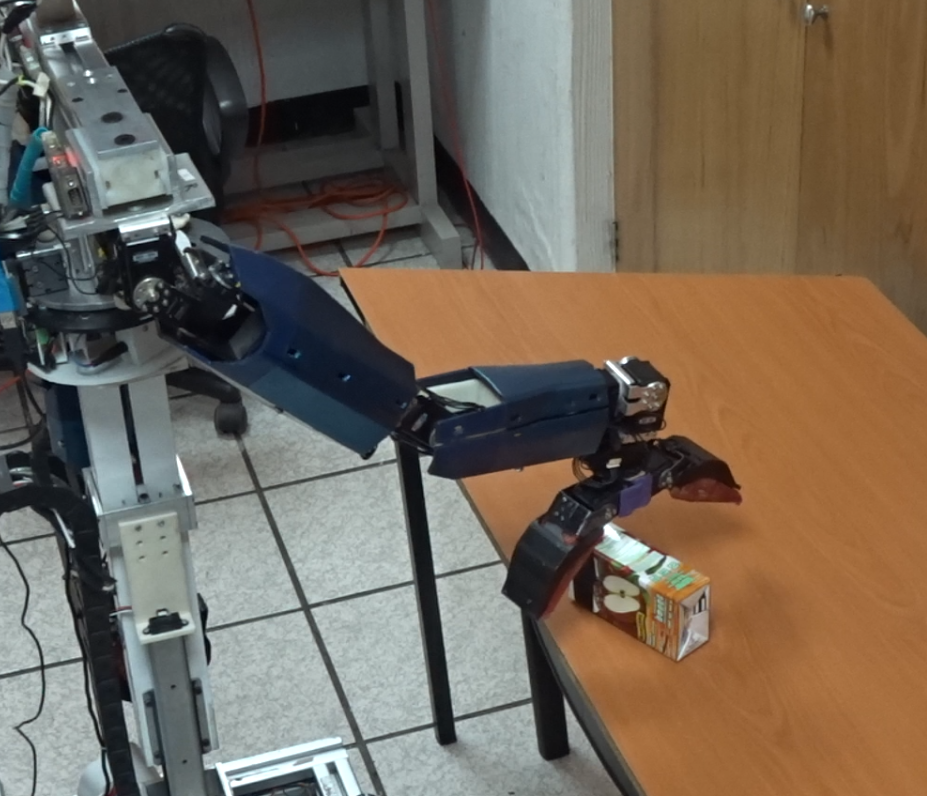
\includegraphics[scale=0.17]{objs_real/juice_success_1.png}
			\caption{Caja de jugo.}
		\end{subfigure}%
		\begin{subfigure}[t]{.55\textwidth}
			\centering
			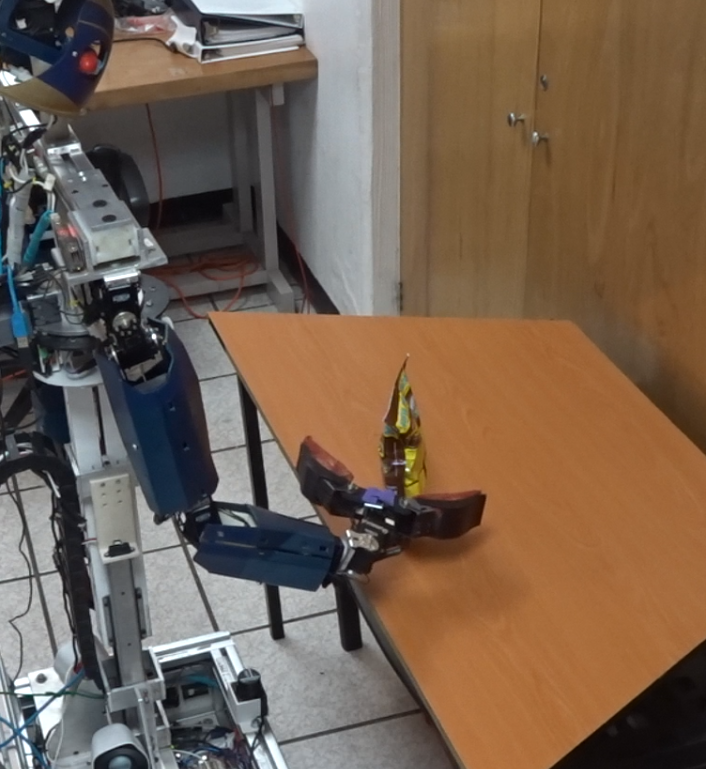
\includegraphics[scale=0.22]{objs_real/cereal_bag_1.png}
			\caption{Cereal.}
		\end{subfigure}
		\caption{Robot Justina realizando la tarea de manipulación con información de orientación.}
		\label{fig:maniOrientation}
		\end{figure}

	Los resultados se muestran en una tabla de éxitos contra fracasos para cada una de las implemetaciones. Posteriormenete se muestra la gráfica \ref{fig:exitos-fracasos} donde se refleja el porcentaje de éxitos para la tarea de toma de objetos.\\

	\begin{table}[H]
		\centering
		\begin{tabular}{ |p{2.8cm}|p{0.4cm}|p{0.4cm}|p{0.4cm}|p{0.4cm}|p{0.4cm}|p{0.4cm}|p{0.4cm}|p{0.4cm}|p{0.4cm}|p{0.4cm}|  }
		\hline
		\multicolumn{11}{|c|}{\textbf{Pruebas de manipulación sin considerar  } }\\
		\multicolumn{11}{|c|}{\textbf{información de orientación (Estado actual) } }\\
		 \hline
		 & \multicolumn{10}{|c|}{\textbf{Eventos} }\\
		 \hline
		  Cereal & $\bigtriangleup$ & $\times$ & $\times$ & $\times$ & $\times$& $\times$ & $\times$ & $\times$ & $\times$ & $\times$ \\
		 \hline
		  Jugo   & $\times$ & $\bigtriangleup$ & $\bigtriangleup$ & $\bigtriangleup$ & $\times$ & $\bigtriangleup$ & $\times$ & $\bigtriangleup$ & $\bigtriangleup$ & $\times$\\
		 \hline
		  Leche  & $\bigtriangleup$ & $\bigtriangleup$ & $\times$ & $\times$ & $\bigtriangleup$ & $\times$ & $\bigtriangleup$  & $\bigtriangleup$ & $\bigtriangleup$ & $\bigtriangleup$\\
		 \hline 
		  Control de videojuegos & $\times$ & $\times$ & $\times$ & $\times$ & $\times$ & $\times$ & $\times$ & $\times$ & $\times$ & $\times$ \\
		 \hline
		  Barra de chocolate     & $\times$ & $\times$ & $\times$ & $\times$ & $\times$ & $\times$ & $\times$ & $\times$ & $\times$ & $\times$\\
		 \hline
		  Libro   & $\times$ & $\times$ & $\times$ & $\times$ & $\times$ & $\times$ & $\times$ & $\times$ & $\times$ & $\times$\\
		 \hline
		 Bolsa de cartón  & $\times$ & $\times$ & $\times$ & $\times$ & $\bigtriangleup$ & $\times$ & $\times$ & $\times$ & $\times$ & $\times$\\
		 \hline
		\end{tabular}
		\caption{Tabla de éxitos-fracasos para la tarea de manipulación de objetos \textbf{(Sin información de orientación)}.}
		\label{t_test:1}
	\end{table}


	\begin{table}[H]
		\centering
		\begin{tabular}{ |p{2.8cm}|p{0.4cm}|p{0.4cm}|p{0.4cm}|p{0.4cm}|p{0.4cm}|p{0.4cm}|p{0.4cm}|p{0.4cm}|p{0.4cm}|p{0.4cm}|  }
		\hline
		\multicolumn{11}{|c|}{\textbf{Pruebas de manipulación con información } }\\
		\multicolumn{11}{|c|}{\textbf{ de orientación (Implementación) } }\\
		 \hline
		 & \multicolumn{10}{|c|}{\textbf{Eventos} }\\
		 \hline
		  Cereal & $\bigtriangleup$ & $\bigtriangleup$ & $\bigtriangleup$ & $\bigtriangleup$ & $\times$& $\bigtriangleup$ & $\times$ & $\bigtriangleup$ & $\times$ & $\times$ \\
		 \hline
		  Jugo   & $\times$ & $\bigtriangleup$ & $\bigtriangleup$ & $\bigtriangleup$ & $\bigtriangleup$ & $\bigtriangleup$ & $\bigtriangleup$ & $\times$ & $\bigtriangleup$ & $\bigtriangleup$\\
		 \hline
		  Leche  & $\bigtriangleup$ & $\bigtriangleup$ & $\bigtriangleup$ & $\times$ & $\bigtriangleup$ & $\bigtriangleup$ & $\bigtriangleup$ & $\times$ & $\bigtriangleup$ & $\bigtriangleup$\\
		 \hline 
		  Control de videojuegos & $\bigtriangleup$ & $\bigtriangleup$ & $\bigtriangleup$ & $\times$ & $\times$ & $\bigtriangleup$ & $\bigtriangleup$ & $\times$ & $\bigtriangleup$ & $\bigtriangleup$ \\
		 \hline
		  Barra de chocolate     & $\bigtriangleup$ & $\bigtriangleup$ & $\bigtriangleup$ & $\bigtriangleup$ & $\times$ & $\bigtriangleup$ & $\times$ & $\bigtriangleup$ & $\bigtriangleup$ & $\times$\\
		 \hline
		  Libro   & $\bigtriangleup$ & $\bigtriangleup$ & $\bigtriangleup$ & $\bigtriangleup$ & $\times$ & $\bigtriangleup$ & $\times$ & $\bigtriangleup$ & $\times$ & $\bigtriangleup$\\
		 \hline
		 Bolsa de cartón  & $\bigtriangleup$ & $\bigtriangleup$ & $\times$ & $\bigtriangleup$ & $\bigtriangleup$ & $\bigtriangleup$ & $\times$ & $\bigtriangleup$ & $\bigtriangleup$ & $\bigtriangleup$\\
		 \hline
		\end{tabular}
		\caption{Tabla de éxitos-fracasos para la tarea de manipulación de objetos \textbf{(Con información de orientación)}}
		\label{t_test:1}
	\end{table}

		

	\begin{figure}[H]
	\hspace*{-0.3in}
	\centering
	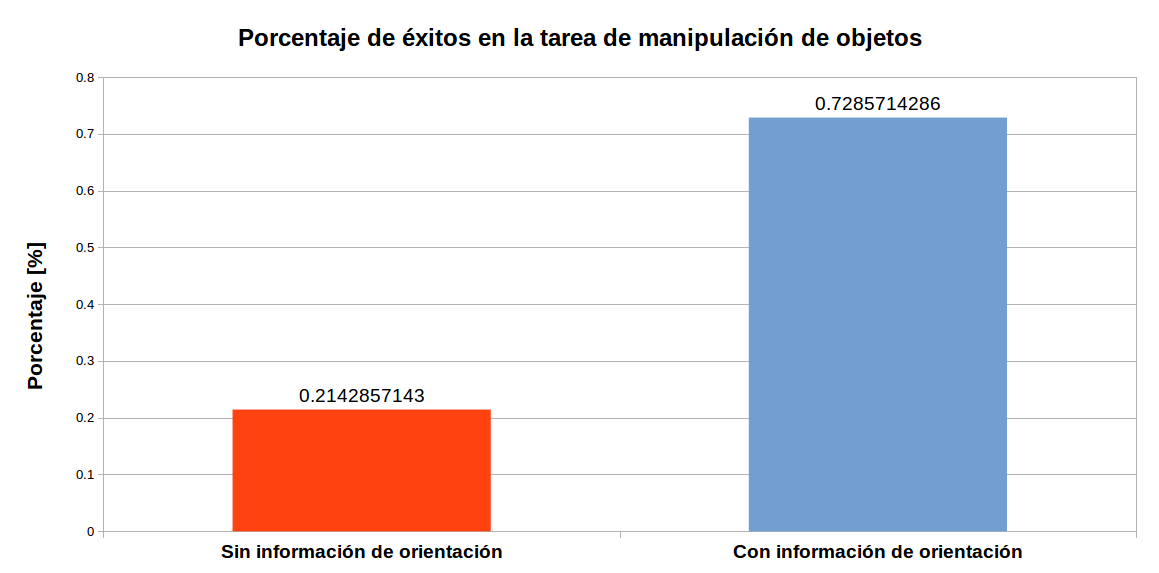
\includegraphics[scale=0.45]{resultados/exitos_graspTask.png}
	\caption{Gráfica comparativa de éxitos fracasos con información de orientación y sin información de la orientación de los oobjetos.}
	\label{fig:exitos-fracasos}
	\end{figure}



\newpage
\thispagestyle{empty}
\mbox{}
\addtocounter{page}{-2}


%%%%%%%%%%%%%%%%%%%%%%%%%%%%%%%%%%%%%%%%%%%%%%%%%%%%%%%%%%%%
%%%%%%%%%		Conclusiones           %%%%%%%%%%%%%%%%%%%%%
\chapter{Conclusiones y trabajo futuro}

\section{Conclusiones} 
	Partiendo de la información obtenida de los resultados podemos concluir que un algoritmo RANSAC con un umbral de 0.02 [m] y un número de 1000 iteraciones nos ayudará a encontrar la ecuación de un plano así como una lista de puntos pertenecientes al mismo. Esta impletenación tomará 8 veces más tiempo que la implementación actual pero reducirá el error relativo respecto al modelo real de un 39.9\% al 8.83\%.\\

	El análisis de componentes principales aplicado a nubes de puntos de objetos segmentados ayuda a cálcular el ángulo de orientación de un objeto sobre el plano.\\

	Inlcuir información sobre la orientación de los objetos a la tarea de manipulación mejora de un 21.4\% a un 72.8\%. Por lo tanto podemos decir que inluir esta información mejora significativamenta la tarea de manipulación para un robot de servicio con un manipulador de 7DOF como Justina.\\   


\section{Trabajo futuro}
